\documentclass[9pt, landscape, a4paper]{article}

\usepackage{Cheatsheet}

% ============= DOCUMENT CONTENT =============

\begin{document}
\pdftitle{Thermodynamics}
\vspace*{-.5cm}
\setlength{\columnsep}{0.5cm}

\begin{multicols*}{3}
\raggedcolumns
\vspace*{-.7cm}
\part{Heat transfer}
\section*{Symbology}
\begin{center}
  \begin{tabular}{cll}
    Symbol & Quantity & Unit \\
    $\lambda$ , $k$ & Thermal conductivity & $\mathrm{W/(m\cdot K)}$ \\
    $\dot{q}$ & Heat flux & $\mathrm{W/m^2}$ \\
    $\dot{Q}$ & Heat flow & $\mathrm{W}$ \\
    $\alpha$ & Heat transfer coefficient & $\mathrm{W/(m^2\cdot K)}$ \\
    $a$ & Thermal diffusivity & $\mathrm{m^2/s}$ \\
    $\nu$ & Kinematic viscosity & $\mathrm{m^2/s}$
  \end{tabular}
\end{center}

\section{Types of heat transfer}
\subsection{Heat conduction}
Occurs with all materials when there is a temperature gradient.

\textbf{Steady-state conduction (1st Fourier's law)}:
\begin{gather*}
  \dot{q} = -\lambda\der{T}{x}
\end{gather*}

\textbf{Transient conduction (2nd Fourier's law 1D)}:
\begin{gather*}
  \dfrac{\partial T}{\partial t} = \dfrac{\lambda}{\rho c_p} \dfrac{\partial^2 T}{\partial x^2}
\end{gather*}

\subsection{Convective heat transfer}
This occurs in moving fluids.

\textbf{Newton's approach}:
\begin{gather*}
  \dot{q} = \alpha\left(T_1 - T_2\right) = \dfrac{\lambda_\text{fluid}}{\delta_\text{th}}\left(T_1 - T_2\right)
\end{gather*}

\subsection{Radiation}
Bodies with a temperature above 0 K emit thermal radiation.
\[\dot{q}_\text{rad} = \epsilon \cdot \sigma \cdot \left(T^4 - T_\infty^4\right)\]

where $\sigma$ is the Stefan-Boltzmann constant:\\
$\sigma = 5.67\cdot 10^{-8}\ \left[\frac{W}{m^2K^4}\right]$

\section{Heat conduction and conductivity}
\subsection{Heat flux}
\begin{gather*}
  \dot{q} = -\lambda\der{T}{x} = k\Delta T = \dfrac{\lambda}{\delta}\Delta T
\end{gather*}
Procedure:
\begin{gather*}
  \vec{\dot{q}} \integral[0][\delta][][x] = -\lambda \integral[T_1][T_2][][T] \Longrightarrow \dot{q} = \dfrac{\lambda}{\delta}\left(T_1 - T_2\right) 
\end{gather*}

\subsection{Heat flow}
\begin{gather*}
  \dot{Q} = \dfrac{\Delta Q}{\Delta t} = \dot{q}A = kA\Delta T = \dfrac{\lambda}{\delta}A\Delta T
\end{gather*}

\subsection{Thermal conduction $k^{-1}$ and Thermal conductivity $k$}
\begin{gather*}
  k^{-1}_\text{tot} = \sum_{i=1}^n \dfrac{\delta_i}{\lambda_i}\ \Longrightarrow\ k_\text{tot} = \dfrac{1}{k^{-1}_\text{tot}}
\end{gather*}

\section{Heat conduction through a hollow cylinder}
\begin{gather*}
  \dot{Q} = -\lambda A \der{T}{r} = -\lambda 2\pi r l \der{T}{r}\\
\end{gather*}
\vspace*{-.9cm}
\figbox{$\dot{Q} = 2\pi l \cdot \dfrac{T_0 - T_1}{\dfrac{1}{\lambda} \ln\dfrac{r_1}{r_0}} = 2\pi r_0 l k \Delta T$}

With multilayered walls:
\begin{gather*}
  \dot{Q} = 2\pi l \cdot \dfrac{T_0 - T_n}{\dm \sum_{i=1}^n \dfrac{1}{\lambda_i} \ln\dfrac{r_i}{r_{i-1}}} = \boxed{2\pi r_0 l k_0 (T_0 - T_n)}
\end{gather*}

\subsection{Thermal conductivity $k$}
\begin{gather*}
  k_0 = \dfrac{1}{r_0\left(\left(\frac{1}{\lambda_1} \ln\frac{r_1}{r_0}\right) + \left(\frac{1}{\lambda_2} \ln\frac{r_2}{r_1}\right) + \dots + \left(\frac{1}{\lambda_n} \ln\frac{r_n}{r_{n-1}}\right)\right)}\\[.3cm]
  k_0^{-1} = r_0\sum_{i=1}^{n}\left(\frac{1}{\lambda_i}\ln\frac{r_i}{r_{i-1}}\right)
\end{gather*}

\subsection{Thin-walled pipe approximated as a flat wall}
\begin{gather*}
  \dot{Q}_T = \lambda A \dfrac{T_0 - T_1}{\delta}\quad ; \quad A = 2\pi l \left(r_0 + \frac{\delta}{2}\right)\\
  \dfrac{\dot{Q}_T}{\dot{Q}_W} = \dfrac{\delta}{\left(r_0 + \frac{\delta}{2}\right)\ln\left(1+\frac{\delta}{r_0}\right)} = \dfrac{\delta}{r_0} \dfrac{1}{\left(1+\frac{\delta}{2r_0}\right) \ln\left(1+\frac{\delta}{r_0}\right)}
\end{gather*}

\section{Convective heat transfer}
\subsection{Reynolds number}
It compares inertial to viscous forces.

\begin{minipage}{0.5\linewidth}
  \centering
  \figbox{$Re = \rho\, c\, \dfrac{L_\text{char}}{\eta} = c\, \dfrac{L_\text{char}}{\nu}$}
\end{minipage}%
\begin{minipage}{0.5\linewidth}
  $Re < 2300$: Laminar flow;\\
  $Re \approx 2300$: Transition zone;\\
  $Re > 2300$: Turbulent flow
\end{minipage}

\subsection{Prandtl number}
It compares momentum diffusivity to thermal diffusivity.\\
Relates the relative thickness of the velocity and thermal boundary layers.
\begin{gather*}
  Pr = \dfrac{\nu}{a} = \dfrac{\delta_\text{fluid}}{\delta_\text{th}} = \dfrac{\eta c_p}{\lambda}\quad ; \quad a = \dfrac{\lambda}{\rho c_p} \quad ; \quad \nu = \dfrac{\eta}{\rho}
\end{gather*}

\subsection{Nusselt number}
Measures convective heat transfer relative to pure conduction across a boundary layer
and the heat transfer coefficient $\alpha$.
\begin{gather*}
  Nu = \dfrac{\alpha\cdot L_\text{char}}{\lambda_\text{fl}} = \dot{q}\dfrac{L_\text{char}}{\lambda\Delta T_\text{char}}\\[.2cm]
  \alpha = \dfrac{Nu\cdot \lambda}{L_\text{char}}
\end{gather*}

\subsubsection{Forced convection}
\figbox{$Nu = c\cdot Re^m \cdot Pr^n$}
where $c$ is a constant.

For laminar flow over a flat plate:
\[Nu = 0.664 \cdot \sqrt{Re} \cdot \sqrt[3]{Pr}\]

For a flow in the transition zone (Tz):
\[Nu_\text{ Tz} = \sqrt{Nu_{\text{ lam}}^2 + Nu_{\text{ turb}}^2}\]

\subsection{Grashof number}
It compares buoyancy to viscous forces.
\begin{gather*}
  Gr = g\beta\Delta T \dfrac{L^3}{\nu^2}\quad ; \quad g = 9.81 \text{ N/kg}\\
  \beta\Delta T = \dfrac{\rho_\infty - \rho_0}{\rho_\infty} = \dfrac{\Delta\rho}{\rho_\infty}\\
  Gr = g\dfrac{\rho_\infty - \rho_0}{\rho_\infty} \dfrac{L^3}{\nu^2}
\end{gather*}

\subsubsection{Natural convection}
\textbf{Peclet number}\\
It compares advective to diffusive heat transport, i.e., the strength of convection relative to thermal diffusion.
\[Pe = Re Pr\]

\textbf{Rayleigh number}\\
It combines buoyancy driving and thermal diffusion, and it measures the intensity of natural convection.
\[Ra = Gr Pr\]

\section{Heat exchanger}
\subsection{Energy balance}
\begin{gather*}
  \dot{Q} = \dot{m}c_p\Delta\vartheta =CP\Delta\vartheta\\
  \dot{Q}_1 = \dot{Q}_2\\
  \dot{m}_1 c_{p1} \Delta\vartheta_1 = \dot{m}_2 c_{p2} \Delta\vartheta_2 \Longleftrightarrow CP_1 \Delta\vartheta_1 = CP_2 \Delta\vartheta_2
\end{gather*}

\subsection{Average temperature difference}
\begin{center}
  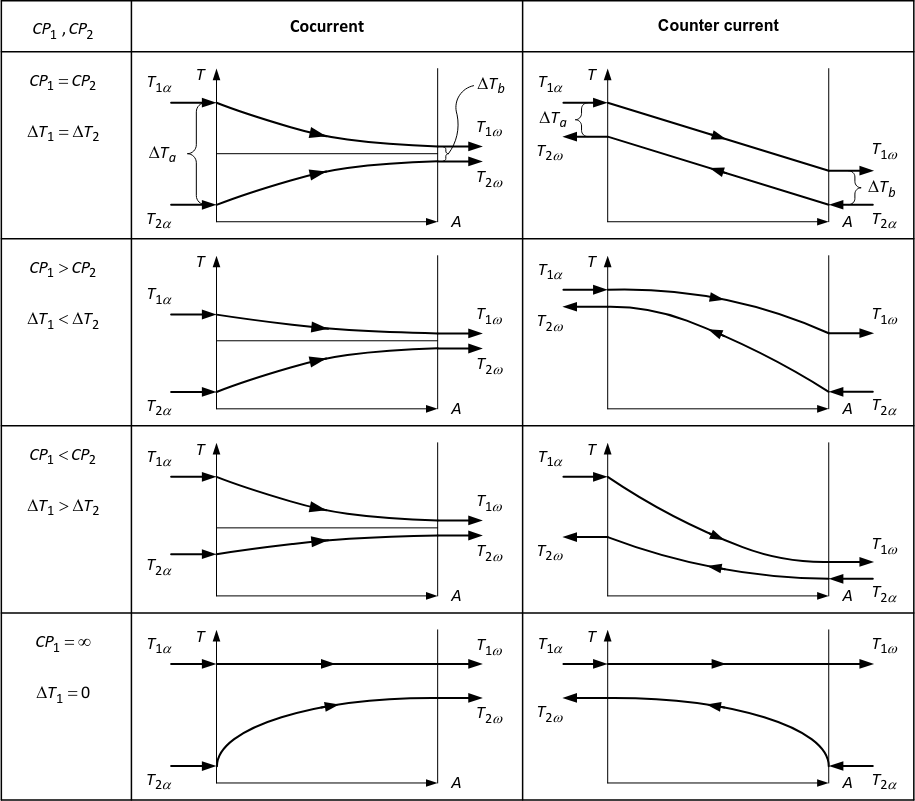
\includegraphics[width=\linewidth]{media/heatexchangers.png}
\end{center}

\subsubsection{Logarithmic mean temperature difference (LMTD)}
\figbox{$\dm \Delta T_m = \dfrac{\Delta T_a - \Delta T_b}{\ln\dfrac{\Delta T_a}{\Delta T_b}}$}
\[\Delta T_a = \left|\vartheta_{1,a} - \vartheta_{2,a}\right|\quad ; \quad \Delta T_b = \left|\vartheta_{1,b} - \vartheta_{2,b}\right|\]

\subsubsection{Mean temperature heat flow}
\figbox{$\dot{Q} = kA\Delta T_m$}

\subsubsection{Heat capacity rate ratio (Capacity ratio)}
It measures the relative ability of stream 1 vs. stream 2 to carry
heat per kelvin:
\begin{gather*}
  CP_1 \left(\vartheta_{1, \alpha} - \vartheta _{1, \omega}\right) = CP_2 \left(\vartheta_{2\omega} - \vartheta_{2,\alpha}\right)\\[1ex]
  R_1 = \dfrac{CP_1}{CP_2} = \dfrac{\vartheta_{2,\omega} - \vartheta_{2,\alpha}}{\vartheta_{1,\alpha}-\vartheta_{1,\omega}} = \dfrac{\Delta \vartheta_2}{\Delta \vartheta_1}
\end{gather*}

\subsection{Co-current vs countercurrent flow heat exchanger}
\begin{gather*}
  \dot{Q} = kA_\text{co}\Delta T_{m,\text{co}} = kA_\text{count}\Delta T_{m,\text{count}}\\
  \dfrac{A_\text{co}}{A_\text{count}} = \dfrac{\Delta T_{m,\text{count}}}{\Delta T_{m,\text{co}}}\\[1ex]
  \dfrac{A_\text{co}}{A_\text{count}} = \dfrac{\dot{Q}_\text{co}}{\dot{Q}_\text{count}}\cdot \dfrac{\Delta T_{m,\text{count}}}{\Delta T_{m,\text{co}}},\quad \text{if } \dot{Q}_1 \neq \dot{Q}_2
\end{gather*}

\newcolumn
\vspace*{-.7cm}
\part{The 2nd law of thermodynamics}
\section{Recap of the 1st law}
\subsection{Closed systems}
\[q_{12} + w_{12} = u_2 - u_1\]

\subsection{Open systems}
\begin{gather*}
  q_{12} + w_{12} = h_2 - h_1 + \dfrac{1}{2}\left(c_2^2 - c_1^2\right) + g\left(z_2 - z_1\right)\\
  w_{t12} = \integral[v][p] + \dfrac{1}{2}\left(c_2^2 - c_1^2\right) + g\left(z_2 - z_1\right) + j_{12}\\
  q_{12} + \integral[v][p] + j_{12} = h_2 - h_1 \overset{\text{ideal gas}}{\xlongequal{\hspace{18pt}}} c_p\left(T_2 - T_1\right)
\end{gather*}

\section{The 2nd law}
\subsection{Statements}
\figbox{Energy = Exergy + Anergy}

\begin{center}
  \begin{tabular}{|c|c|c|}
    \hline \textbf{Processes}& \textbf{Reversible} & \textbf{Irreversible}\\
    \hline \textbf{Exergy} & Conserved & Reduced $\rightarrow$ Loss\\
    \hline \textbf{Entropy} & Constant & Increases $\rightarrow$ Production\\
    \hline
  \end{tabular}
\end{center}

\subsection{Entropy}
Entropy $S$: extensive state variable [J/K]\\[1ex]
Specific entropy $s$: intensive state variable [J/kgK]\\[1ex]
Entropy flow $\dot{S}$: entropy over time [W/K]

\section{Entropy balance equation}
\figbox{\[dS = dS_Q + dS_m + dS_{irr}\]}

\subsection{Entropy balance terms}
\begin{itemize}
    \item Heat transfer across the system boundary:
    \[dS_Q = \frac{dQ}{T}\]
    \item Mass flow across the system boundary:
    \[dS_{\mathrm{m}} = \dot{m}\,s\ dt\quad ; \quad \dot{S}_m = \dot{m}\,s\]
    \item Irreversible processes inside the system:
    \[\dot{S}_{irr}(t)\begin{cases}
      dS_{irr} > 0 &\text{ irreversible processes}\\
      dS_{irr} = 0 &\text{ reversible processes}\\
      dS_{irr} < 0 &\text{ impossible}
    \end{cases}\]
\end{itemize}

\subsection{Entropy balance equation for closed systems}
\begin{gather*}
  dS = dS_Q + \cancelto{0}{dS_m} + dS_{irr}\\
  dS = \dot{S}_Q\ dt + \dot{S}_{irr}\ dt = \left(\dfrac{\dot{Q}}{T} + \dot{S}_{irr}\right) dt 
\end{gather*}

\newcolumn
\subsubsection{Closed system entropy flow balance equation}
\begin{gather*}
  \dfrac{dS}{dt} = \sum_i \dot{S}_{Qi} + \dot{S}_{irr}\quad ; \quad \dot{S}_{irr} \geq 0
\end{gather*}

For steady-state case:
\begin{gather*}
  \dot{S}_{irr} = -\sum_i \dot{S}_{Qi} = -\sum_i \dfrac{\dot{Q}_i}{T_i} \geq 0
\end{gather*}

\subsubsection{Visual representation}
\begin{minipage}{0.5\linewidth}
  \centering
  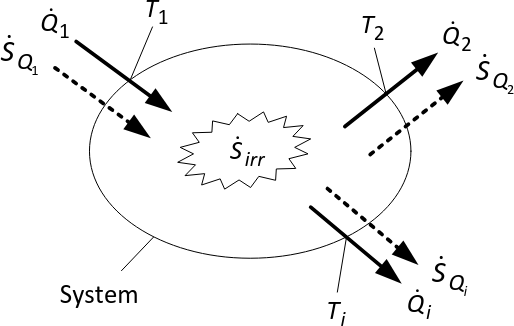
\includegraphics[width=\linewidth]{media/entropy_closedsystem.png}
\end{minipage}%
\begin{minipage}{0.5\linewidth}
  \figbox{$\dm \sum_i \dot{S}_{Qi} = \sum_i\dfrac{\dot{Q}_i}{T_i} = -\dot{S}_{irr}$}
\end{minipage}

\subsection{Entropy balance equation for open systems}
\[\dfrac{dS}{dt} = \sum_\alpha \dot{m}_\alpha s_\alpha - \sum_\omega \dot{m}_\omega s_\omega + \sum \dot{S}_Q(t) + \dot{S}_{irr}(t)\]

\subsubsection{Steady-state flow processes}
\[\dot{S}_{irr} = \sum_\omega \dot{m}_\omega s_\omega - \sum_\alpha \dot{m}_\alpha s_\alpha - \sum \dot{S}_Q \geq 0\]

\subsubsection{Steady-state and adiabatic flow processes}
\[\dot{S}_{irr} = \sum_\omega \dot{m}_\omega s_\omega - \sum_\alpha \dot{m}_\alpha s_\alpha \geq 0\]

\section{The thermal engine}
\begin{minipage}{0.4\linewidth}
  \centering
  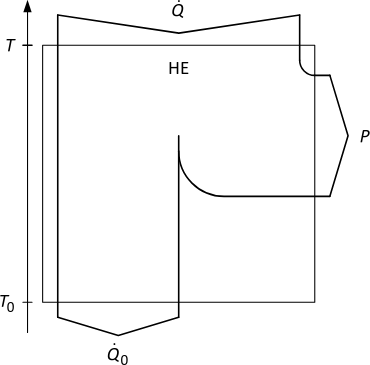
\includegraphics[width=\linewidth]{media/thermal_engine.png}
\end{minipage}%
\begin{minipage}{0.6\linewidth}
  \begin{align*}
    &\dot{Q}+\dot{Q}_0 + P = 0\\
    &\eta_{th} = \dfrac{-P}{\dot{Q}} = 1 - \dfrac{\left|\dot{Q}_0\right|}{\dot{Q}}\\
    &\dot{S}_{irr} = -\sum_{i=1}^{n} \dot{S}_{Qi} = -\dfrac{\dot{Q}}{T} - \dfrac{\dot{Q}_0}{T_0} \geq 0\\
    &-\dot{Q}_0 = T_0\left(\dfrac{\dot{Q}}{T} + \dot{S}_{irr}\right)
  \end{align*}
\end{minipage}

\subsection{Carnot efficiency}
\begin{gather*}
  \eta_{th} = 1 - \dfrac{T_0}{T} - \cancelto{0,\text{ ideal}}{\dfrac{T_0 \dot{S}_{irr}}{\dot{Q}}}\\
  \eta_{th,max} = \eta_C(T,T_0) = 1 - \dfrac{T_0}{T}
\end{gather*}

\newpage
\section{Entropy $S$ as a state variable}
\begin{gather*}
  ds = \dfrac{dq + dj}{T} = \dfrac{du + p\ dv}{T} = \dfrac{dh - v\ dp}{T}\\
  T\ ds = dq + dj \Longrightarrow T\left(s_2 - s_1\right) = q_{12} + j_{12}\\
  \text{General form: } \integral[1][2][T][s] = q_{12} + j_{12}
\end{gather*}

\subsection{Reversible processes}
\subsubsection{Clausius entropy relation}
\figbox{$\delta q_{\mathrm{rev}} = T\,ds \Longleftrightarrow \delta Q_\mathrm{rev} = T\, dS$}

\subsubsection{Work $W$ and heat $Q$}
\begin{gather*}
  w_{p,\ rev} = \integral[v][p]\\
  Q_{rev} = \integral[T][S]
\end{gather*}

\subsection{Dissipation $j$ as a state variable}
\subsubsection{Dissipation}
\begin{gather*}
  w_{t12} = w_{p12} + j_{12} \Longleftrightarrow w_{p12} = w_{t12} - j_{12}\\
  dq_{rev} + dw_{v,\ rev} = du\\
  T\ ds = dq + T\ ds_{irr} = dq_{rev} + dj\\
  \integral[1][2][T][s] = q_{12} + j_{12}
\end{gather*}

\subsubsection{For closed systems}
\begin{gather*}
  ds = \dfrac{du + p\ dv}{T} = \dfrac{c_v\ dT}{T} + \dfrac{R_i\ dv}{v}\\[1ex]
  \boxed{s_2 - s_1 = c_v \ln \dfrac{T_2}{T_1} + R_i \ln \dfrac{v_2}{v_1}}
\end{gather*}

\subsubsection{Work change}
All the works can be calculated with a temperature change:
\begin{gather*}
  q_{12} + w_{t12} = h_2 - h_1 + \dfrac{c_2^2 - c_1^2}{2} + g\left(z_2 - z_1\right)\\
  q_{12} + \integral[v][p] + j_{12} = h_2 - h_1 = c_p\left(T_2 - T_1\right)\\
  \integral[T][s] = q_{12} + j_{12} = \boxed{\integral[T][s] + \integral[v][p] = h_2 - h_1}\\
  \boxed{T\ ds + v\ dp = h_2 - h_1 \Longleftrightarrow T\ ds - p\ dv = u_2 - u_1}\\
  T\, ds + v\, dp = dh\, T\, ds - p\, dv = du
\end{gather*}

\newcolumn
\subsection{Reversible state changes with perfect gases}
\subsubsection{Open system}
\begin{gather*}
  q_{12} + j_{12} + w_{p,rev} = h_2 - h_1\\
  \integral[1][2][T][s] + \integral[1][2][v][p] = c_p\left(T_2 - T_1\right)
\end{gather*}

\subsubsection{Closed system}
\begin{gather*}
  q_{12} + j_{12} + w_{v,rev} = u_2 - u_1\\
  \integral[1][2][T][s] - \integral[1][2][p][v] = c_v\left(T_2 - T_1\right)
\end{gather*}

\subsection{Polytropic state changes}
\begin{gather*}
  T\ ds = dq + dj = du + p\ dv = dh - v\ dp\\
  du + p\ dv = c_v\ dT + p\ dv \quad ; \quad dh - v\ dp = c_p\ dT - v\ dp\\
  dw_v = c_v \frac{k-1}{n-1}\ dT = -p\ dv
\end{gather*}

For the change in entropy of the polytropic state change:
\begin{gather*}
  ds = c_v \dfrac{n-k}{n-1} \dfrac{dT}{T}\\[1ex]
  \frac{T_2}{T_1} = \left(\dfrac{v_1}{v_2}\right)^{n-1} = \left(\dfrac{p_2}{p_1}\right)^{\frac{n-1}{n}}\\[1ex]
  \boxed{s_2 - s_1 = c_v \dfrac{n - k}{n-1} \ln \dfrac{T_2}{T_1}}\quad n\neq 1\\[1ex]
  \boxed{s_2 - s_1 = c_v \ln\dfrac{T_2}{T_1} + R_i \ln\dfrac{v_2}{v_1} = c_p \ln\dfrac{T_2}{T_1} - R_i \ln\dfrac{p_2}{p_1}}
\end{gather*}

\textbf{Compressor with dissipation}: $n > k$\\
\textbf{Turbine with dissipation}: $n < k$

\section{Exergy and anergy}
\textbf{Exergy}: useful part of energy that can be completely converted into work under given ambient conditions.\\[1ex]
\textbf{Anergy}: remaining part of energy that cannot be converted into work under given ambient conditions.
\figbox{$e = ex + an$}

\subsection{Statements of the 2nd LT}
\begin{enumerate}[label=\textbf{\Roman*.}]
  \item In all irreversible processes exergy is converted into anergy
  \item Only in reversible processes exergy remains constant
  \item It is impossible to convert anergy into exergy
\end{enumerate}

\subsection{Exergy}
\subsubsection{Exergy balance / Exergy loss}
\begin{center}
  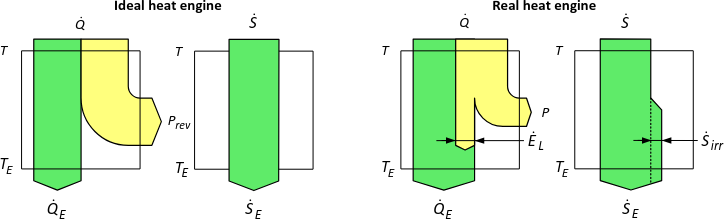
\includegraphics[width=\linewidth]{media/exergy.png}
\end{center}
\begin{gather*}
  \dot{E}_L = \sum_\alpha \dot{E}_\alpha - \sum_\omega |\dot{E}_\omega| = \dot{Q}\dfrac{T_A - T_E}{T_A} + \left(-\dot{Q}\dfrac{T_B - T_E}{T_B}\right)\\
  \boxed{\dot{E}_L = T_E\dot{S}_{irr} = T_E\dfrac{T_A - T_B}{T_AT_B}\dot{Q}}\\
  \dot{S}_{irr} = \sum_\omega \dot{m}_\omega s_\omega - \sum_\alpha \dot{m}_\alpha s_\alpha - \sum \dot{S}_Q \geq 0,\quad d\dot{S}_Q = \dfrac{d\dot{Q}}{T}
\end{gather*}

\subsubsection{Exergy of heat}
\[\dot{E}_Q = P_{rev} = \left(1-\frac{T_E}{T}\right)\dot{Q} = \eta_C \dot{Q}\]

\subsubsection{Exergy of material flows (without mixtures)}
\begin{gather*}
  e = h - h_E - T_E\left(s-s_E\right) + \dfrac{c^2}{2} + gz + q\left(1-\dfrac{T_E}{T}\right)\\[1ex]
  \boxed{e_2 - e_1 = h_2 - h_1 - T_E\left(s_2 - s_1\right)}
\end{gather*}

\pph{Perfect gases}
\begin{gather*}
  e = c_p\left(T - T_E - T_E \ln\dfrac{T}{T_E}\right) + R_i T_E \ln\dfrac{p}{p_E}
\end{gather*}

\pph{Incompressible liquids (isobaric)}
\[e = c_p\left(T - T_E - T_E\ln\dfrac{T}{T_E}\right)\]

\pph{Isobaric for $T < T_E$ (cooling)}
\[e = c_p\left(T_E - T - T_E\ln\dfrac{T_E}{T}\right)\]
\vfill \phantom{}

\newcolumn
\vspace*{-.7cm}
\part{Steady-state flow processes}
\section{Adiabatic working cycles}
\subsection{Compressor}
\subsubsection{1st law}
\begin{gather*}
  w_{t12} + q_{12} = h_2 - h_1 + \dfrac{1}{2}\left(c_2^2 - c_1^2\right) + g\left(z_2 - z_1\right)\\
  w_{t12} + q_{12} = c_p\left(T_2 - T_1\right) + \dfrac{1}{2}\left(c_2^2 - c_1^2\right) + g\left(z_2 - z_1\right)\\
  P_{12} + \dot{Q}_{12} = \dot{m}\left(w_{t12} + q_{12}\right)
\end{gather*}

\subsubsection{Isentropic compression efficiency factor}
\begin{gather*}
  \eta_s = \dfrac{\text{isentropic work}}{\text{real polytropic work}}\\[1.5ex]
  \eta_s = \dfrac{\Delta h_s}{\Delta h} = \dfrac{h_{2,s} - h_1}{h_2 - h_1} = \dfrac{c_{p,m} \left(T_{2,s} - T_1\right)}{c_{p,m} \left(T_2 - T_1\right)} = \dfrac{T_{2,s} - T_1}{T_2 - T_1} \leq 1
\end{gather*}

\subsection{Turbine}
\subsubsection{1st law}
\begin{gather*}
  w_{t12} + q_{12} = h_2 - h_1 + \dfrac{1}{2}\left(c_2^2 - c_1^2\right) + g\left(z_2 - z_1\right)\\
  w_{t12} + q_{12} = c_p\left(T_2 - T_1\right) + \dfrac{1}{2}\left(c_2^2 - c_1^2\right) + g\left(z_2 - z_1\right)\\
  P_{12} = \dot{m}w_{t12} \Longleftrightarrow -P_{12} = \dot{m}\left|w_{t12}\right|
\end{gather*}

\subsubsection{Isentropic turbine efficiency}
\begin{gather*}
  \eta_s = \dfrac{\text{real polytropic work}}{\text{isentropic work}}\\[1.5ex]
  \eta_s = \dfrac{-\Delta h}{-\Delta h_s} = \dfrac{h_1 - h_2}{h_1 - h_{2,s}} = \dfrac{T_1 - T_2}{T_1 - T_{2,s}}
\end{gather*}

\section{Adiabatic flow processes without work}
\subsection{Throttle / Expansion valve (isenthalpic)}
\begin{gather*}
  h_1 = h_2 \Longrightarrow j_{12} = -\integral[1][2][v][p] = -R_i T \ln\dfrac{p_2}{p_1}
\end{gather*}

\subsection{Nozzle}
\begin{gather*}
  h_2^0 = h_1^0 \Longrightarrow h_2 + \dfrac{1}{2}c_2^2 = h_1 + \dfrac{1}{2}c_1^2\\
  c_2 = \sqrt{2\left(h_1 - h_2\right) + c_1^2}
\end{gather*}
where $h^0$ is the total enthalpy: $h^0 = h + \dfrac{c^2}{2}$
\newcolumn

\vspace*{-.6cm}
\part{Thermodynamics cycles}
\section{Reversible cycle work}
Total cycle / sum of all sub-processes:
\figbox{$\dm w_{t,\, rev} = \integral[1][2][v][p] + \integral[2][3][v][p] + \ldots + \integral[n][1][v][p] = \oint v\ dp = \sum_{i=1}^{n} w_{pi}$}

\begin{center}
  \resizebox{0.6\columnwidth}{!}{%
  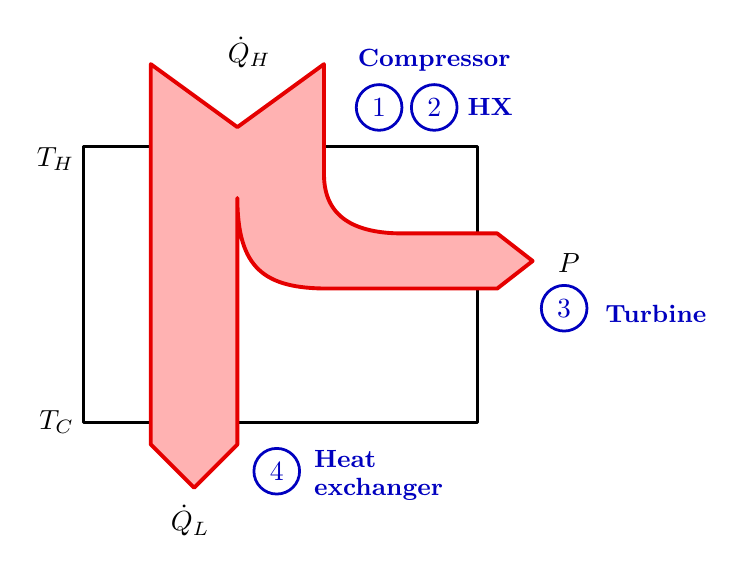
\begin{tikzpicture}[line cap=round, line join=round]
  
    \colorlet{myblue}{blue!75!black}
    \colorlet{myred}{red!90!black}
    
    \draw[black, line width=1.1pt] (0,0) rectangle (5,3.5);
    
    \node[left] at (0,3.35) {$T_H$};
    \node[left] at (0,0.00) {$T_C$};
    
    \draw[myred, line width=1.4pt, fill=red!30]
      (0.85,-0.28) -- (0.85,4.55)
      -- (1.95,3.75)
      -- (3.05,4.55)
      -- (3.05,3.15)
      .. controls (3.05,2.60) and (3.45,2.40) .. (4.05,2.40)
      -- (5.25,2.40)
      -- (5.70,2.05)
      -- (5.25,1.70)
      -- (3.10,1.70)
      .. controls (2.30,1.70) and (1.95,1.95) .. (1.95,2.85)
      -- (1.95,-0.28)
      -- (1.40,-0.83)
      -- cycle;
    
    \node at (2.10,4.7) {$\dot{Q}_H$};
    \node at (1.35,-1.25) {$\dot{Q}_L$};
    \node[right] at (5.9,2.02) {$P$};
    
    \tikzset{
      state/.style={
        draw=myblue, text=myblue, line width=1pt,
        circle, minimum size=5.8mm, inner sep=0pt
      },
      blabel/.style={text=myblue, font=\bfseries\small}
    }
    
    \node[blabel] at (4.45,4.6) {Compressor};
    
    \node[state] at (3.75,4.00) {1};
    \node[state] at (4.45,4.00) {2};
    \node[blabel, anchor=west] at (4.75,4.00) {HX};
    
    \node[state] at (6.10,1.45) {3};
    \node[blabel, anchor=west] at (6.50,1.38) {Turbine};
    
    \node[state] at (2.45,-0.62) {4};
    \node[blabel, anchor=west] at (2.8,-0.47) {Heat};
    \node[blabel, anchor=west] at (2.8,-0.85) {exchanger};
  
  \end{tikzpicture}%
  }
\end{center}

\subsection{Clockwise cycle}
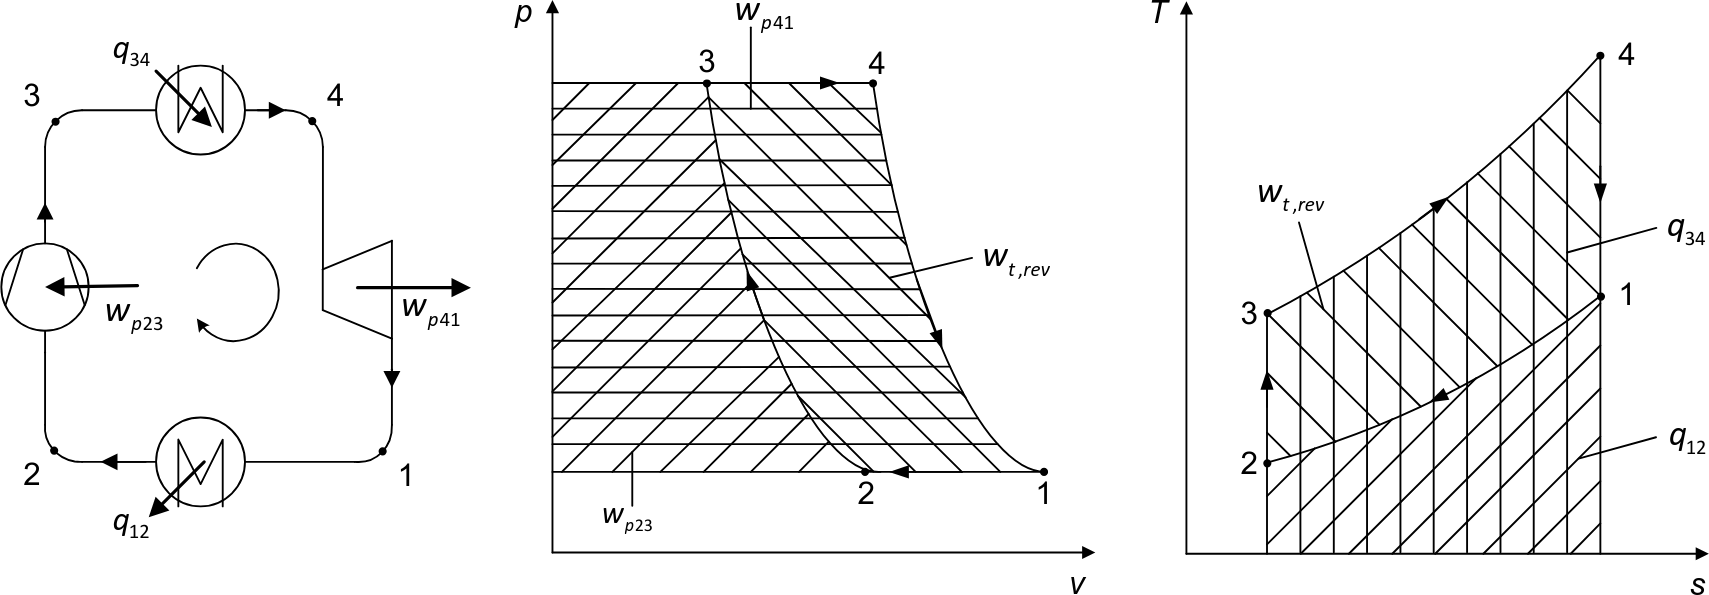
\includegraphics[width=\linewidth]{media/clockwise.png}
\begin{gather*}
  w_{t,rev} = w_{p,23} + w_{p,41} < 0\\
  \left|w_{t,rev}\right| = \left|q_{34}\right| - \left|q_{12}\right|
\end{gather*}

\subsection{Counterclockwise cycle}
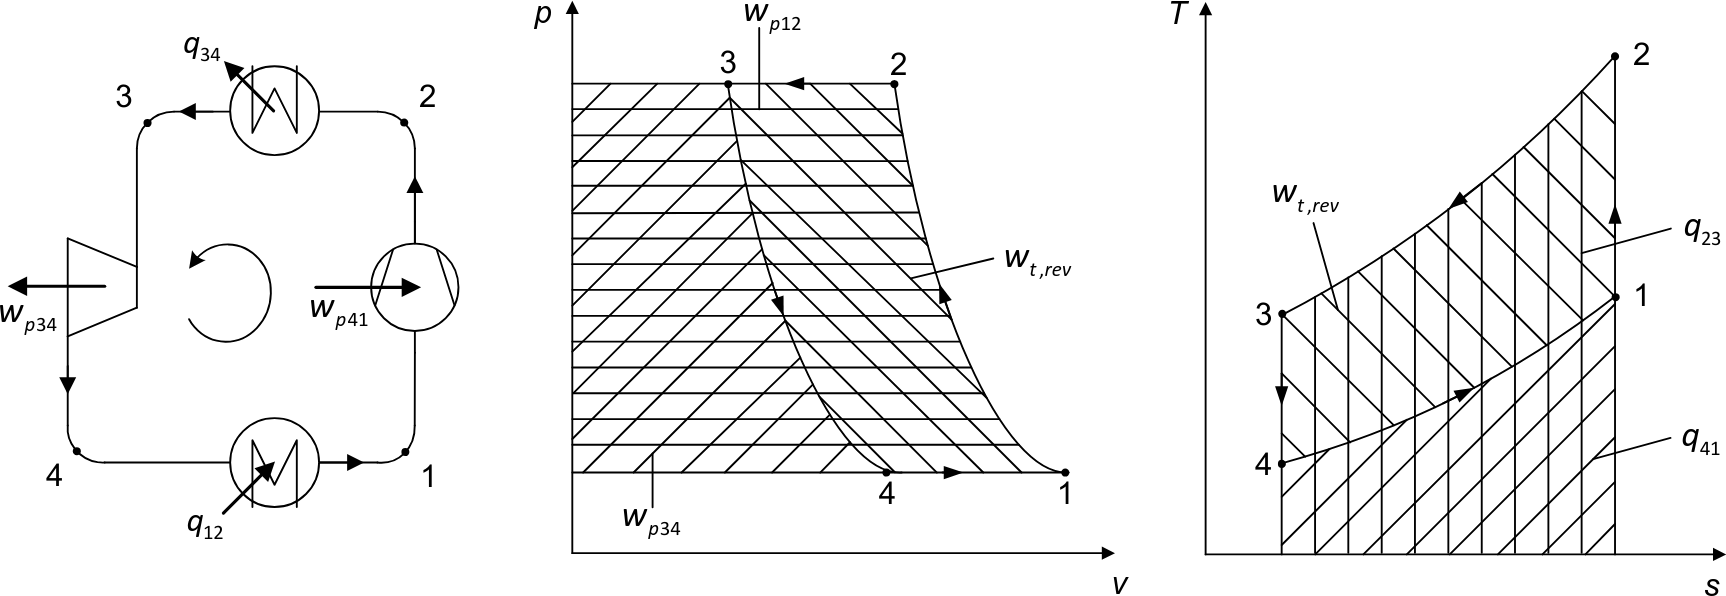
\includegraphics[width=\linewidth]{media/counterclockwise.png}
\begin{gather*}
  w_{t,rev} = w_{p,12} + w_{p,34} < 0\\
  \left|w_{t,rev}\right| = \left|q_{23}\right| - \left|q_{41}\right|
\end{gather*}

\newcolumn
\vspace*{-.6cm}
\part{Thermal systems with gas turbines}
\section{Turbine}
\begin{center}
  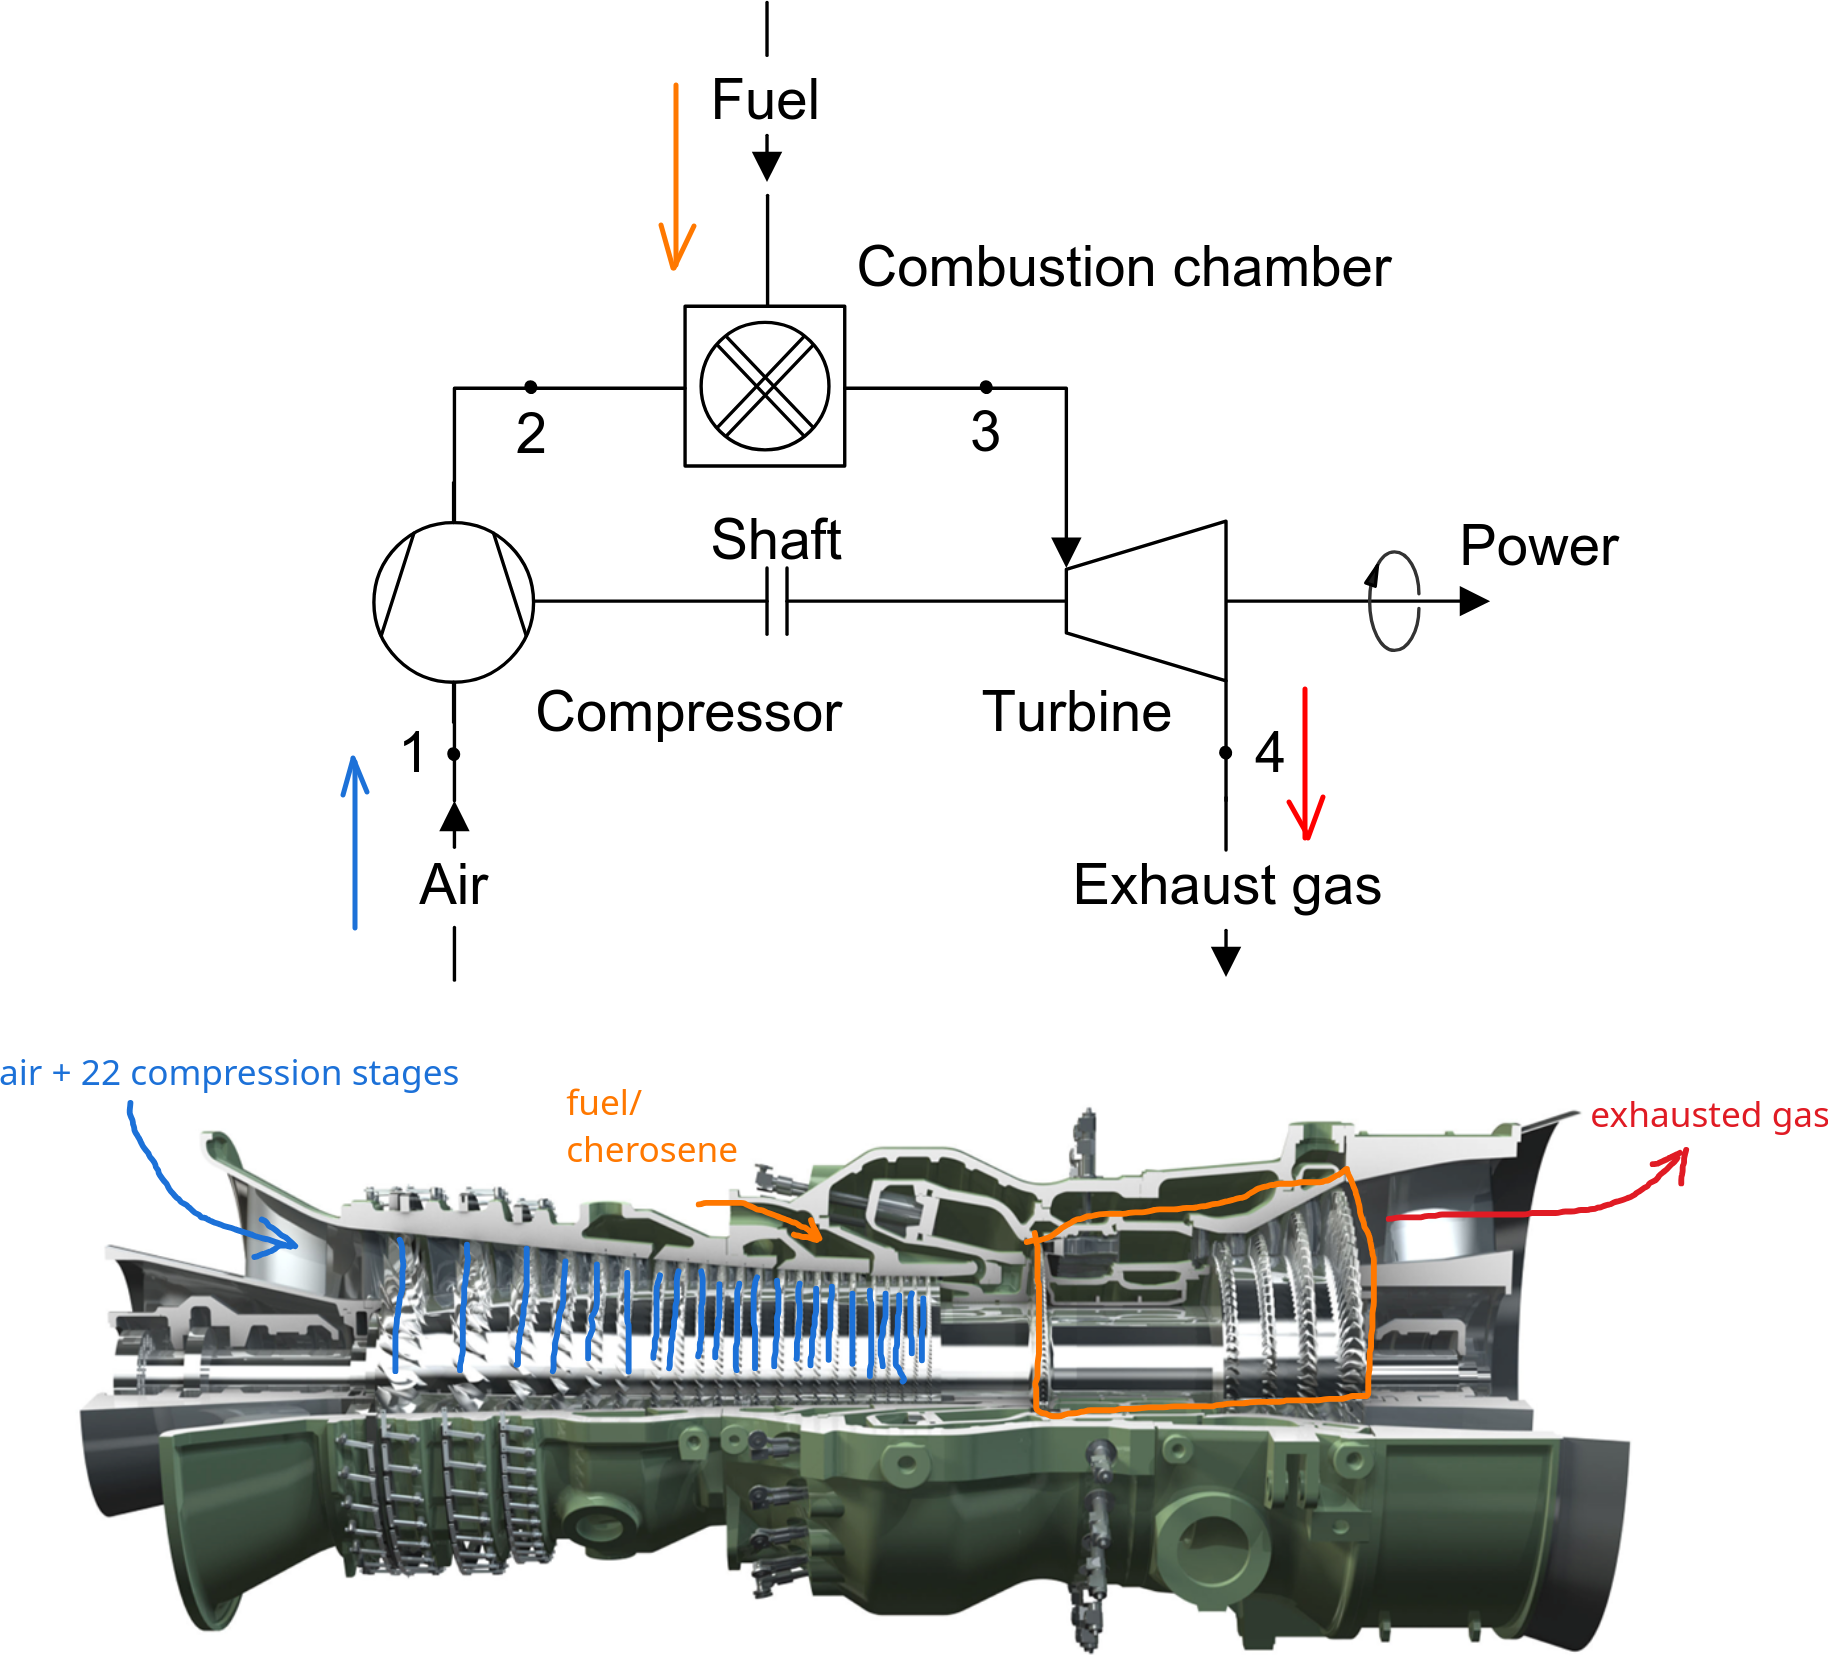
\includegraphics[width=.8\linewidth]{media/turbine.png}
\end{center}
Power balance:
\[\dot{Q}_{23}+\dot{Q}_{41}+P_C = 0\]

\subsection{Joule process}
\begin{gather*}
  \pi = \dfrac{p_2}{p_1} = \dfrac{p_3}{p_4}\\[1ex]
  -w_C = q_\alpha + q_\omega = q_{23} + q_{41} = c_p\left(T_3-T_2+T_1-T_4\right)\\[1ex]
  \left|w_C\right| = c_p\left(T_3-T_2\right)\left(1-\dfrac{T_4-T_1}{T_3-T_2}\right)\\[1ex]
  \dfrac{T_4-T_1}{T_3-T_2} = \left(\dfrac{p}{p_0}\right)^{\frac{k-1}{k}} = \left(\frac{1}{\pi}\right)^{\frac{k-1}{k}}\\[1ex]
  \eta_J = \dfrac{\left|w_C\right|}{q_\alpha} = 1 - \dfrac{T_1}{T_2} = 1 - \left(\dfrac{1}{\pi}\right)^{\frac{k-1}{k}}
\end{gather*}

\newpage
\vspace*{-.6cm}

\part{Thermal plants with steam turbines}
\section{Types of steam}
\begin{center}
  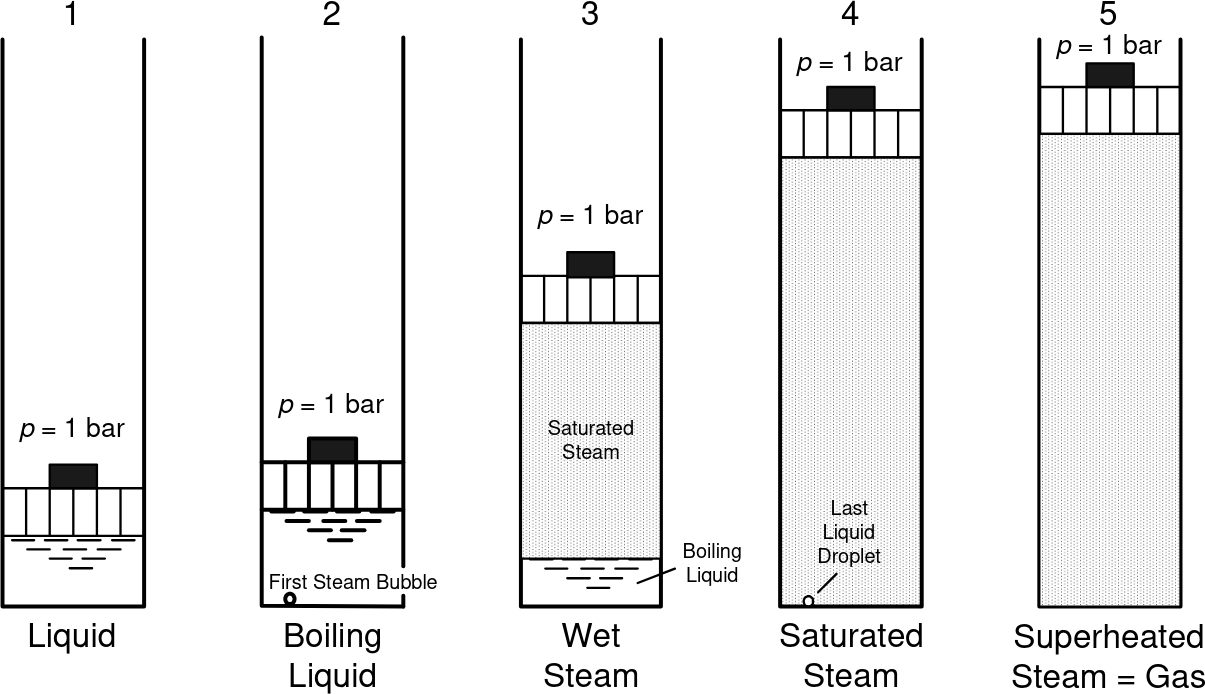
\includegraphics[width=.75\linewidth]{media/steam.png}
\end{center}

\section{Boundary curves of the two phase region}
\begin{center}
  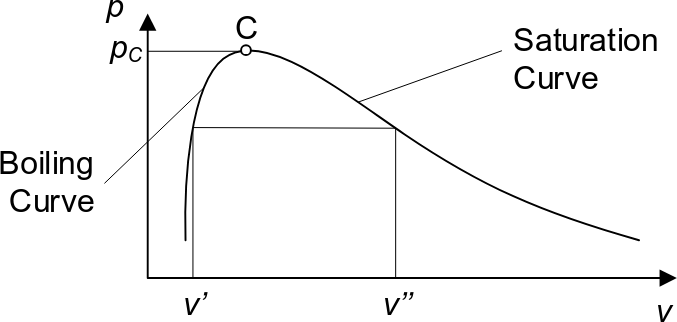
\includegraphics[width=.75\linewidth]{media/boundary_curves.png}
\end{center}

\subsection{Steam tables}
\begin{gather*}
  v = (1-x)v' + xv'' = v' + x(v'' - v')\\[1ex]
  h = (1-x)h' + xh'' = h' + x\Delta h_v\\[1ex]
  s = (1-x)s' + xs'' = s' + x\left(\dfrac{\Delta h_v}{T}\right)
\end{gather*}

\subsubsection{Steam content}
\begin{gather*}
  x = \dfrac{v-v'}{v''-v'}\\[1ex]
  x = \dfrac{h-h'}{h''-h'} = \dfrac{h-h'}{\Delta h_v}\\[1ex]
  x = \dfrac{s-s'}{s''-s'} = (s-s')\dfrac{T}{\Delta h_v}
\end{gather*}

\subsubsection{Subcooling / Condenser enthalpy}
\begin{gather*}
  h_1 = h'([p,t,s]) - c_p \Delta T_\text{subcooling}\\
  \dot Q_\text{heating} = \dot m \cdot c_p \Delta T_\text{heating}
\end{gather*}

\subsection{Water pump}
\[P_\text{el}\cdot \eta_p = \dot m \cdot c_p \cdot \Delta T\]

\newcolumn
\section{Steam power stations}
\subsection{Rankine cycle}
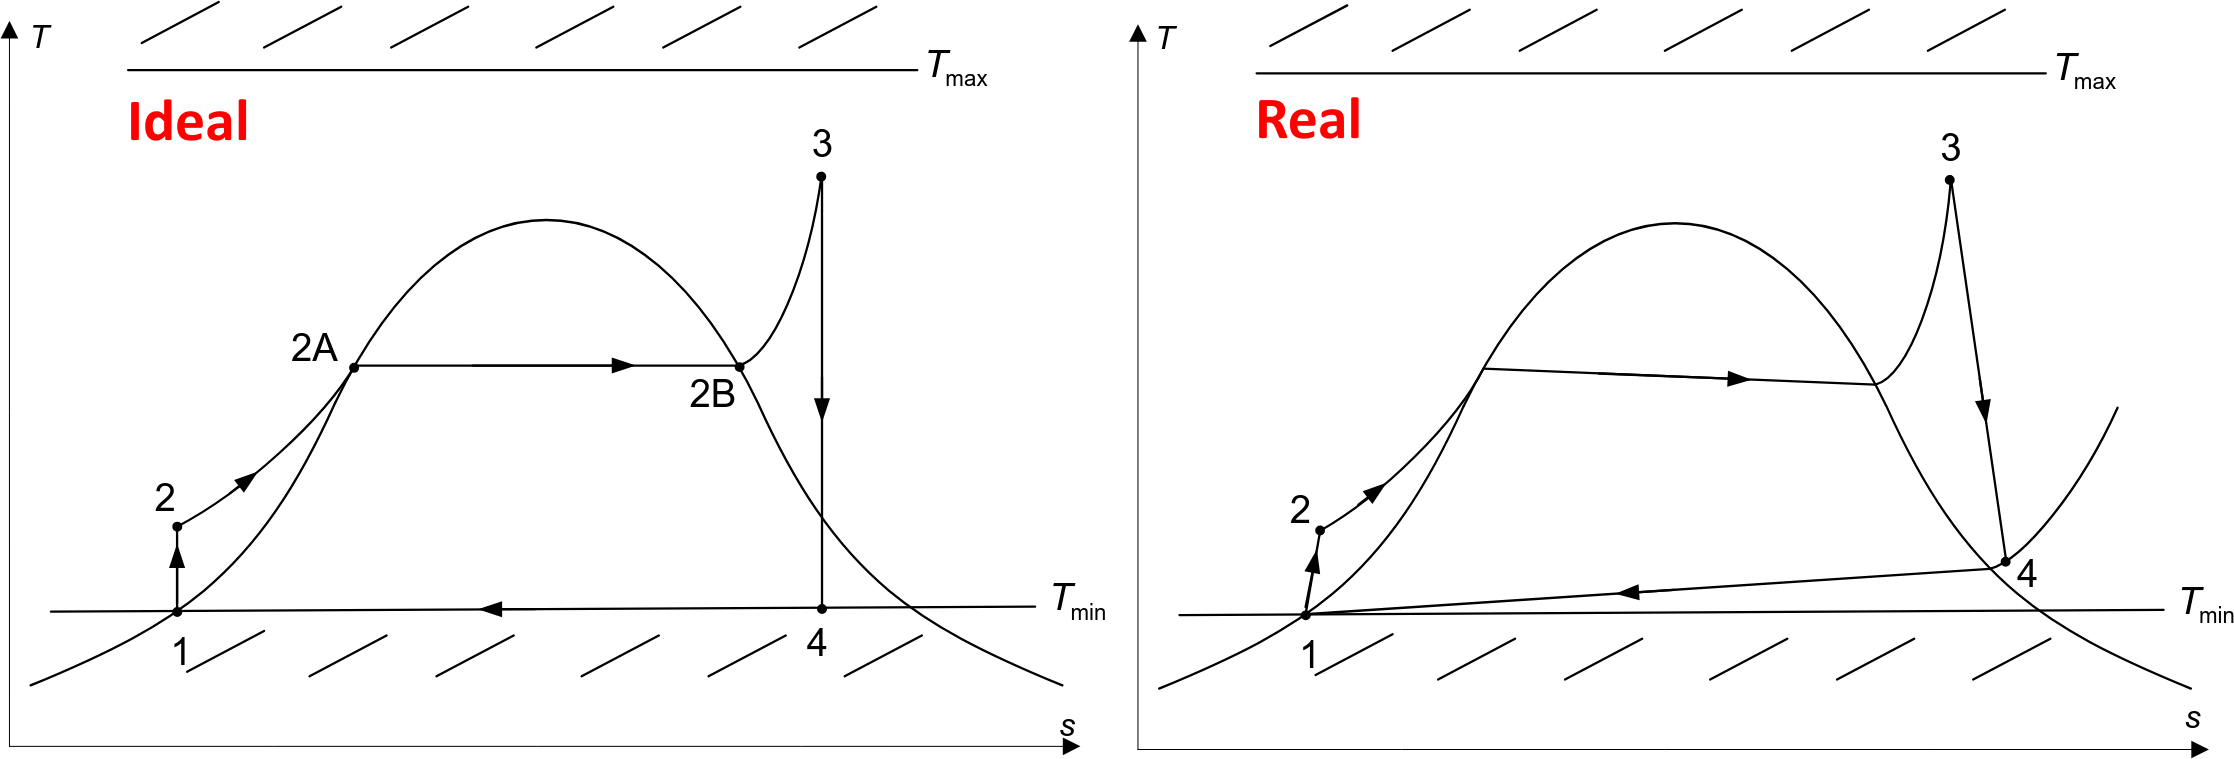
\includegraphics[width=\linewidth]{media/rankine-T-s.png}
\begin{minipage}{.48\linewidth}
  \begin{align*}
    w_{t12} &= h_2 - h_1 \text{ (pump)}\\
    q_{23} &= h_3 - h_2 \text{ (boiler)}
  \end{align*}
\end{minipage}
\hfill
\begin{minipage}{.48\linewidth}
  \begin{align*}
    \left|w_{t34}\right| &= h_3 - h_4 \text{ (turbine)}\\
    \left|q_{41}\right| &= h_4 - h_1 \text{ (condenser)}
  \end{align*}
\end{minipage}

\[\eta_{th} = \dfrac{(h_3 - h_4) \overbrace{- (h_2 - h_1)}^{\text{pump work}}}{h_3 - h_2}\quad ; \quad \eta_s = \frac{h_3 - h_4}{h_3 - h_{4,s}}\leq 1\]

\subsubsection{Generator}
\[P_G = \dot m_D \cdot \left(h_3 - h_4\right) \cdot \prod_i \eta_i\]

\part{Heat pumps and Chillers}
\section{T-s and log p-h diagrams}
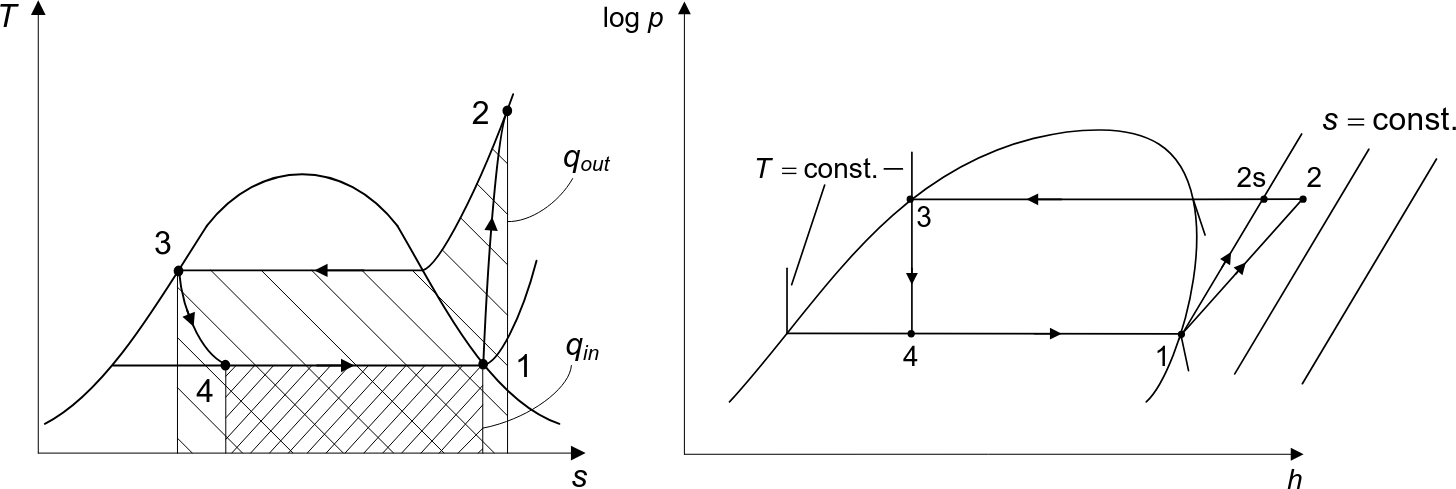
\includegraphics[\lw]{media/heatpump.png}
\begin{minipage}{.48\linewidth}
  \begin{align*}
    w_{t,12} &= h_2 - h_1 \text{ (compressor)}\\
    q_{23} &= h_2 - h_3 \text{ (condenser)}
  \end{align*}
\end{minipage}
\hfill
\begin{minipage}{.48\linewidth}
  \begin{align*}
    h_3 &= h_4 \text{ (expansion valve)}\\
    q_{41} &= h_1 - h_4 \text{ (evaporator)}
  \end{align*}
\end{minipage}

\subsection{Isentropic efficiency (compressor)}
\[\eta_s = \frac{h_{2,s}-h_1}{h_2-h_1} \leq 1\]

\section{Heat pumps (HP)}
\subsection{Inner coefficient of performance}
\begin{gather*}
  \varepsilon_\text{HP} = \frac{\left|q_{23}\right|}{w_{12}} = \frac{\text{heat}}{\text{technical work}} = \frac{h_2-h_3}{h_2-h_1} = \varepsilon_R + 1\\[1ex]
  \text{Carnot: }\frac{1}{\eta_C} = \varepsilon_{HP,C} = \frac{T_C}{T_C - T_E} = \frac{T_C}{\Delta T_\text{lift}} = \varepsilon_{R,C} + 1
\end{gather*}

\subsection{Outer coefficient of performance (COP)}
\begin{center}
  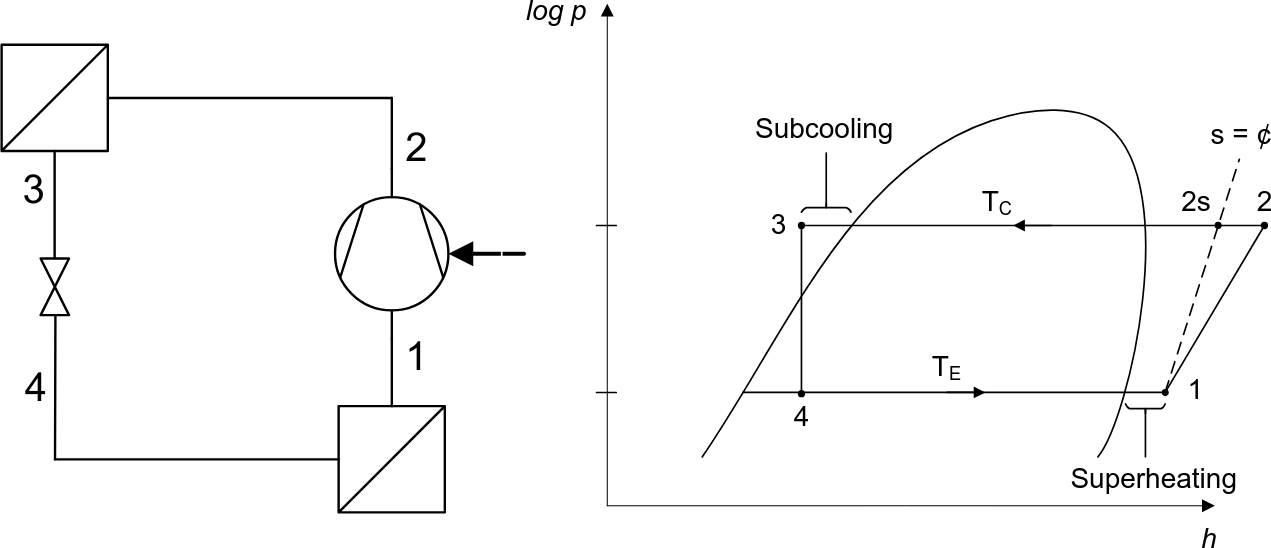
\includegraphics[\lw=.75]{media/heat-pump.png}
\end{center}
\begin{gather*}
  \text{COP}_\text{HP} = \frac{\lvert\dot{Q}_\omega\rvert}{P_{el}} = \frac{\lvert\dot{Q}\rvert}{P_{el}} = \eta_\text{mech}\cdot \varepsilon_\text{HP}\\[1ex]
  \varepsilon_{HP} > COP_{HP} \quad ; \quad \zeta_{HP} = \frac{COP_{HP}}{\varepsilon_{HP,C}}
\end{gather*}

\subsection{Real inner COP}
Assumptions: $\zeta = 0.5,\ \Delta T_e = 10K,\ \Delta T_c = 5K$

\begin{gather*}
  \varepsilon_{HP,C} = \dfrac{\vartheta_\text{req} - \Delta T_c}{\left(\vartheta_\text{env} - \Delta T_c\right) - \left(\vartheta_\text{req} - \Delta T_e\right)}\\[1ex]
  \varepsilon_\text{HP} = \zeta_{HP}\cdot \varepsilon_{HP,C}
\end{gather*}

\section{Chillers / refrigerators (R)}
\subsection{Inner coefficient of performance}
\begin{gather*}
  \varepsilon_R = \frac{\left|q_{41}\right|}{w_{12}} = \frac{h_1-h_4}{h_2-h_1} = \varepsilon_\text{HP} - 1\\[1ex]
  \text{Carnot: } \varepsilon_{R,C} = \frac{T_E}{T_C - T_E} = \frac{T_E}{\Delta T_\text{lift}} = \varepsilon_{HP,C} - 1
\end{gather*}

\subsection{Outer coefficient of performance (COP)}
\begin{gather*}
  EER = COP_R = \dfrac{\dot{Q}_{in}}{P_{el}} = \dfrac{\dot{Q}_e}{P_{el}} = \eta_\text{mech}\cdot \varepsilon_R\\[1ex]
  \varepsilon_R > EER \quad ; \quad \zeta_R = \dfrac{EER}{\varepsilon_{R,C}}
\end{gather*}

\subsection{Real inner COP}
Assumptions: $\zeta = 0.5,\ \Delta T_e = 10K,\ \Delta T_c = 5K$

\begin{gather*}
  \varepsilon_{R,C} = \dfrac{\vartheta_\text{req} - \Delta T_e}{\left(\vartheta_\text{env} - \Delta T_c\right) - \left(\vartheta_\text{req} - \Delta T_e\right)}\\[1ex]
  \varepsilon_R = \zeta_R\cdot \varepsilon_{R,C}
\end{gather*}

\newpage
\vspace*{-.6cm}
\part{Data interpolation and extrapolation}
\section{Interpolation}
For any property $X$, with $X \in \{v,h,s\}$, the general linear interpolation
formula is:
\begin{gather*}
  X = X_1 + \frac{x-x_1}{x_2-x_1}\left(X_2-X_1\right)
\end{gather*}
where $x$ can be pressure, temperature, or another independent variable.

\subsection{Temperature interpolation at constant pressure}

If the pressure is already available in the table, but the required temperature
lies between two tabulated temperatures $\vartheta_1$ and $\vartheta_2$, then:
\begin{gather*}
  v = v_1 + \frac{\vartheta-\vartheta_1}{\vartheta_2-\vartheta_1}
  \left(v_2-v_1\right)\\[1ex]
  h = h_1 + \frac{\vartheta-\vartheta_1}{\vartheta_2-\vartheta_1}
  \left(h_2-h_1\right)\\[1ex]
  s = s_1 + \frac{\vartheta-\vartheta_1}{\vartheta_2-\vartheta_1}
  \left(s_2-s_1\right)
\end{gather*}

\subsection{Pressure interpolation at constant temperature}

If the temperature is already available in the table, but the required pressure
lies between two tabulated pressures $p_1$ and $p_2$, then:
\begin{gather*}
  v = v_{p_1} + \frac{p-p_1}{p_2-p_1}
  \left(v_{p_2}-v_{p_1}\right)\\[1ex]
  h = h_{p_1} + \frac{p-p_1}{p_2-p_1}
  \left(h_{p_2}-h_{p_1}\right)\\[1ex]
  s = s_{p_1} + \frac{p-p_1}{p_2-p_1}
  \left(s_{p_2}-s_{p_1}\right)
\end{gather*}

\subsection{Double interpolation in pressure and temperature}

If both pressure and temperature are between table values, first interpolate
with respect to temperature at $p_1$ and $p_2$, then interpolate with respect
to pressure.

Let: $p_1 < p < p_2 \qquad ; \qquad \vartheta_1 < \vartheta < \vartheta_2$

For any property $X \in \{v,h,s\}$:
\begin{gather*}
  X_{p_1} =
  X_{11} + \frac{\vartheta-\vartheta_1}{\vartheta_2-\vartheta_1}
  \left(X_{12}-X_{11}\right)\\[1ex]
  X_{p_2} =
  X_{21} + \frac{\vartheta-\vartheta_1}{\vartheta_2-\vartheta_1}
  \left(X_{22}-X_{21}\right)\\[1ex]
  X =
  X_{p_1} + \frac{p-p_1}{p_2-p_1}
  \left(X_{p_2}-X_{p_1}\right)
\end{gather*}

\subsection{Saturated steam values}

For saturated steam properties at the top of the steam table, the same pressure
interpolation formula can be used:
\begin{gather*}
  X'' =
  X''_1 + \frac{p-p_1}{p_2-p_1}
  \left(X''_2-X''_1\right)
\end{gather*}
where:
\begin{gather*}
  X'' \in \{v'',h'',s''\}
\end{gather*}

\section{Extrapolation}
For any property $X$, with $X \in \{v,h,s\}$:
\begin{gather*}
  X = X_1 + \frac{x-x_1}{x_2-x_1}\left(X_2-X_1\right)
\end{gather*}
where $x$ is outside the interval $[x_1,x_2]$.

\subsection{Pressure extrapolation at constant temperature}

If the required pressure is outside the tabulated pressure range, use the two
nearest available tabulated pressures. For any property $X \in \{v,h,s\}$:
\begin{gather*}
  X =
  X_{p_1} + \frac{p-p_1}{p_2-p_1}
  \left(X_{p_2}-X_{p_1}\right)
\end{gather*}
where $p$ is outside the interval $[p_1,p_2]$.

For the individual steam-table properties:
\begin{gather*}
  v =
  v_{p_1} + \frac{p-p_1}{p_2-p_1}
  \left(v_{p_2}-v_{p_1}\right)\\[1ex]
  h =
  h_{p_1} + \frac{p-p_1}{p_2-p_1}
  \left(h_{p_2}-h_{p_1}\right)\\[1ex]
  s =
  s_{p_1} + \frac{p-p_1}{p_2-p_1}
  \left(s_{p_2}-s_{p_1}\right)
\end{gather*}

\subsection{Temperature extrapolation at constant pressure}

If the required temperature is outside the tabulated temperature range, use the
two nearest available temperatures. For any property $X \in \{v,h,s\}$:
\begin{gather*}
  X =
  X_1 + \frac{\vartheta-\vartheta_1}{\vartheta_2-\vartheta_1}
  \left(X_2-X_1\right)
\end{gather*}

For the individual properties:
\begin{gather*}
  v =
  v_1 + \frac{\vartheta-\vartheta_1}{\vartheta_2-\vartheta_1}
  \left(v_2-v_1\right)\\[1ex]
  h =
  h_1 + \frac{\vartheta-\vartheta_1}{\vartheta_2-\vartheta_1}
  \left(h_2-h_1\right)\\[1ex]
  s =
  s_1 + \frac{\vartheta-\vartheta_1}{\vartheta_2-\vartheta_1}
  \left(s_2-s_1\right)
\end{gather*}

\subsection{Saturated steam extrapolation}

For saturated steam properties outside the tabulated pressure range:
\begin{gather*}
  X'' =
  X''_1 + \frac{p-p_1}{p_2-p_1}
  \left(X''_2-X''_1\right)
\end{gather*}
where:
\begin{gather*}
  X'' \in \{v'',h'',s''\}
\end{gather*}

For example, using $25$ bar and $50$ bar to estimate the value at $100$ bar:
\begin{gather*}
  X''_{100} = 3X''_{50}-2X''_{25}
\end{gather*}

\end{multicols*}

% ======== PROVIDED FORMULA SHEET =========
\appendix
\clearpage
\section{T-s diagram}
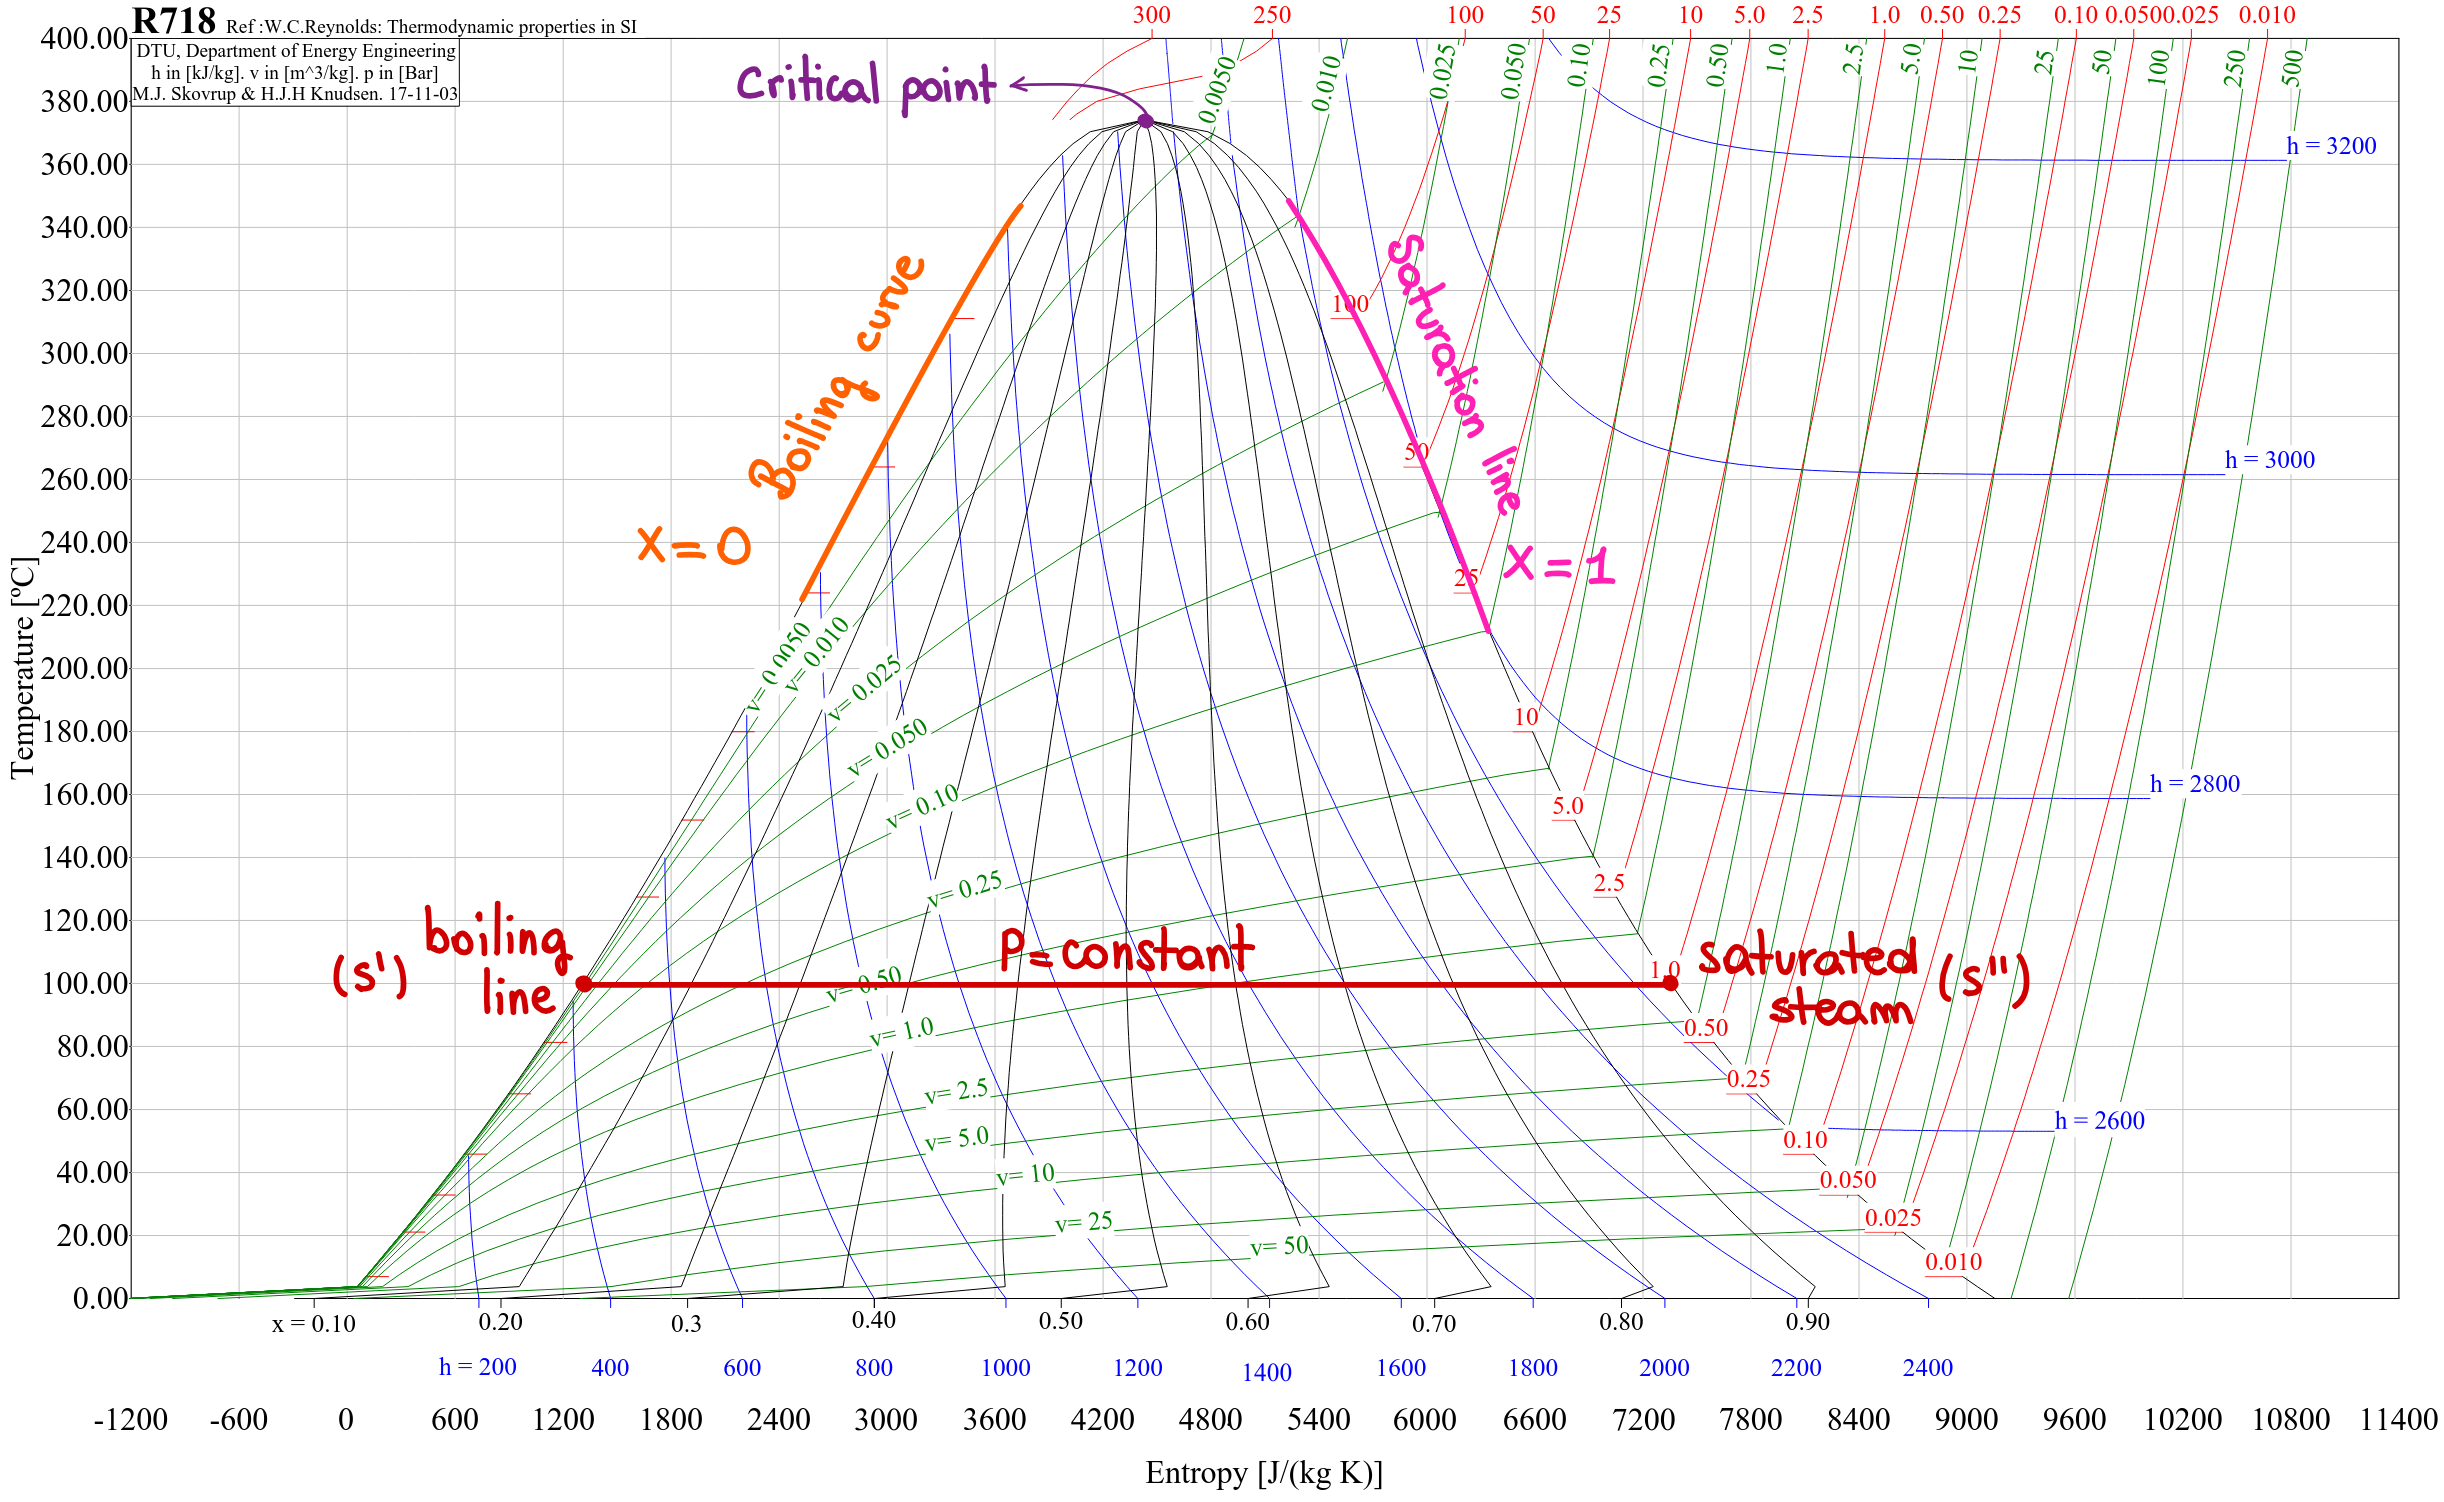
\includegraphics[width=\textwidth]{media/T-s-diagram.png}
\clearpage
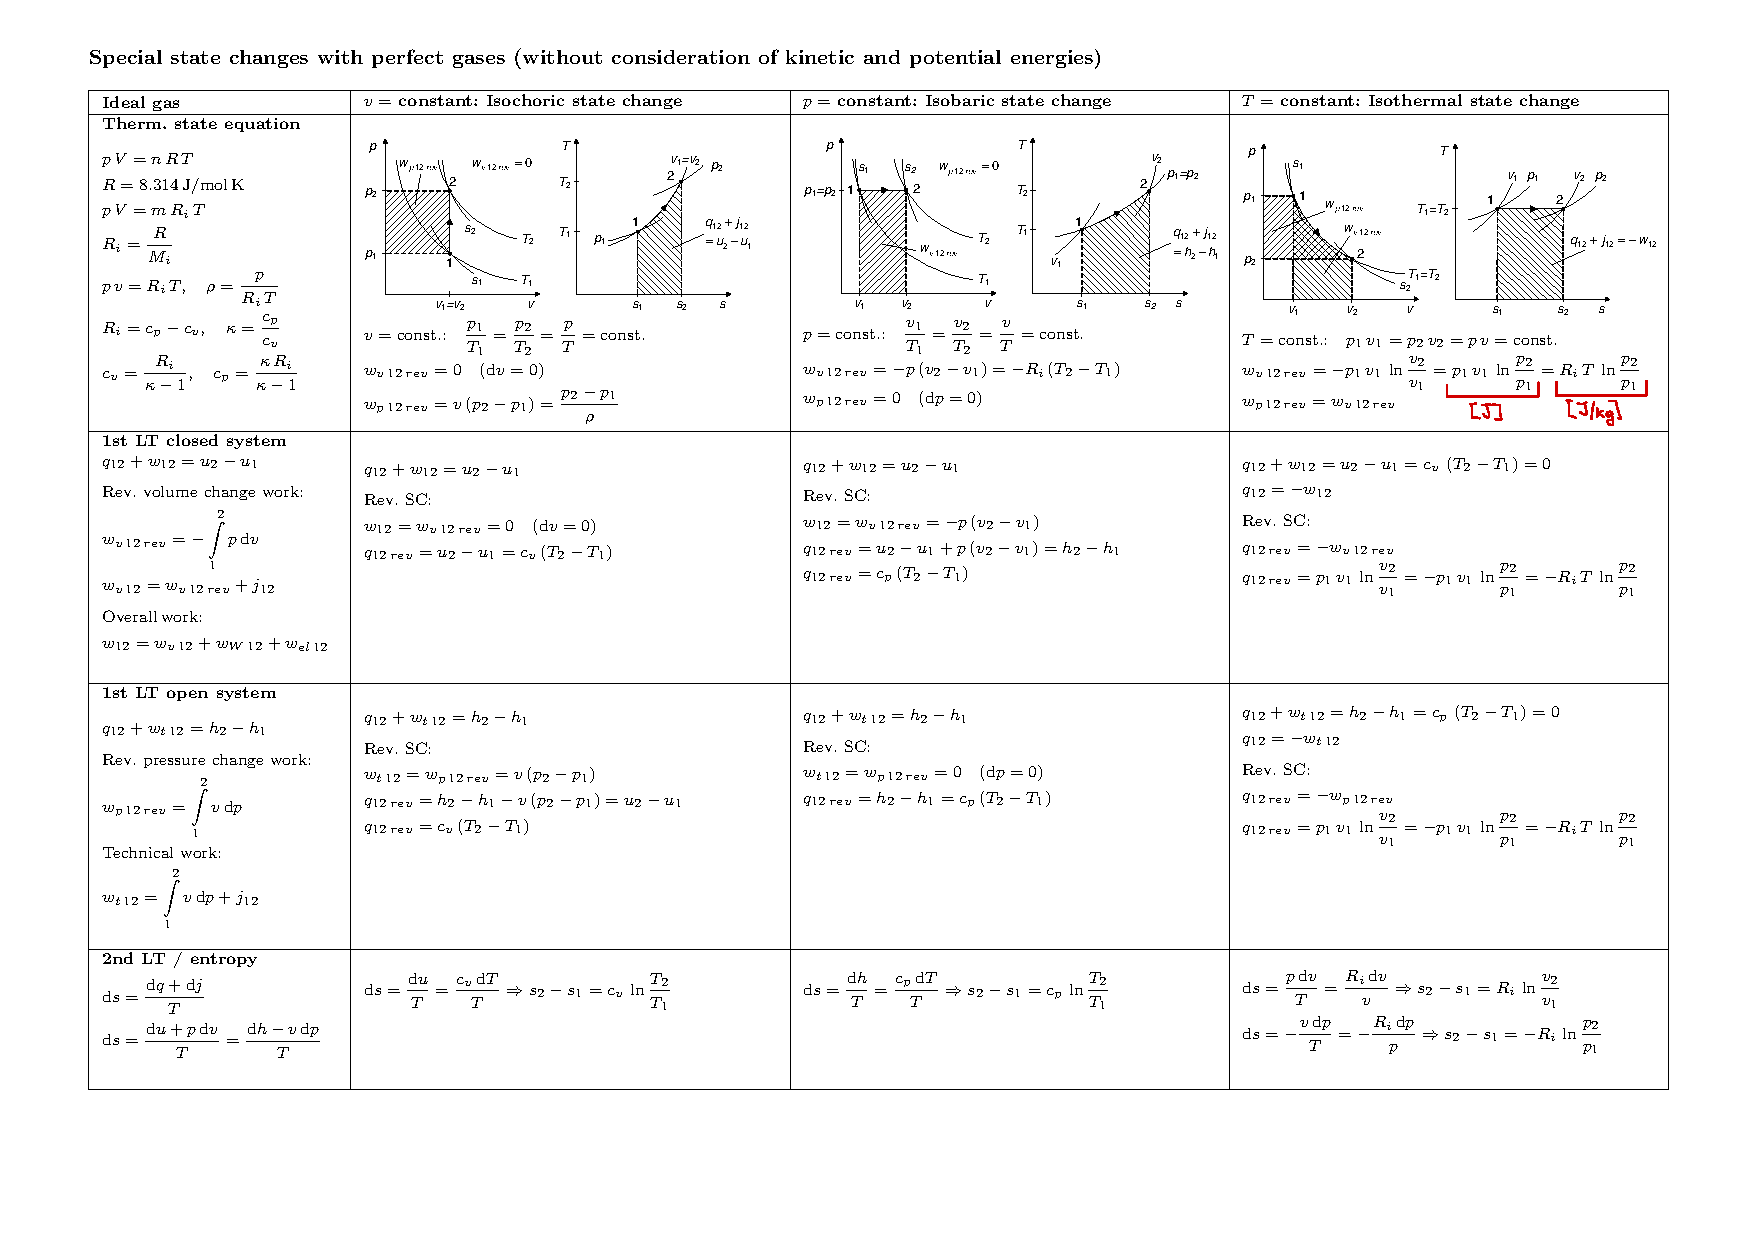
\includepdf[pages=1,pagecommand={\thispagestyle{fancy}}]{media/FormulaSheet-1.pdf}
\clearpage
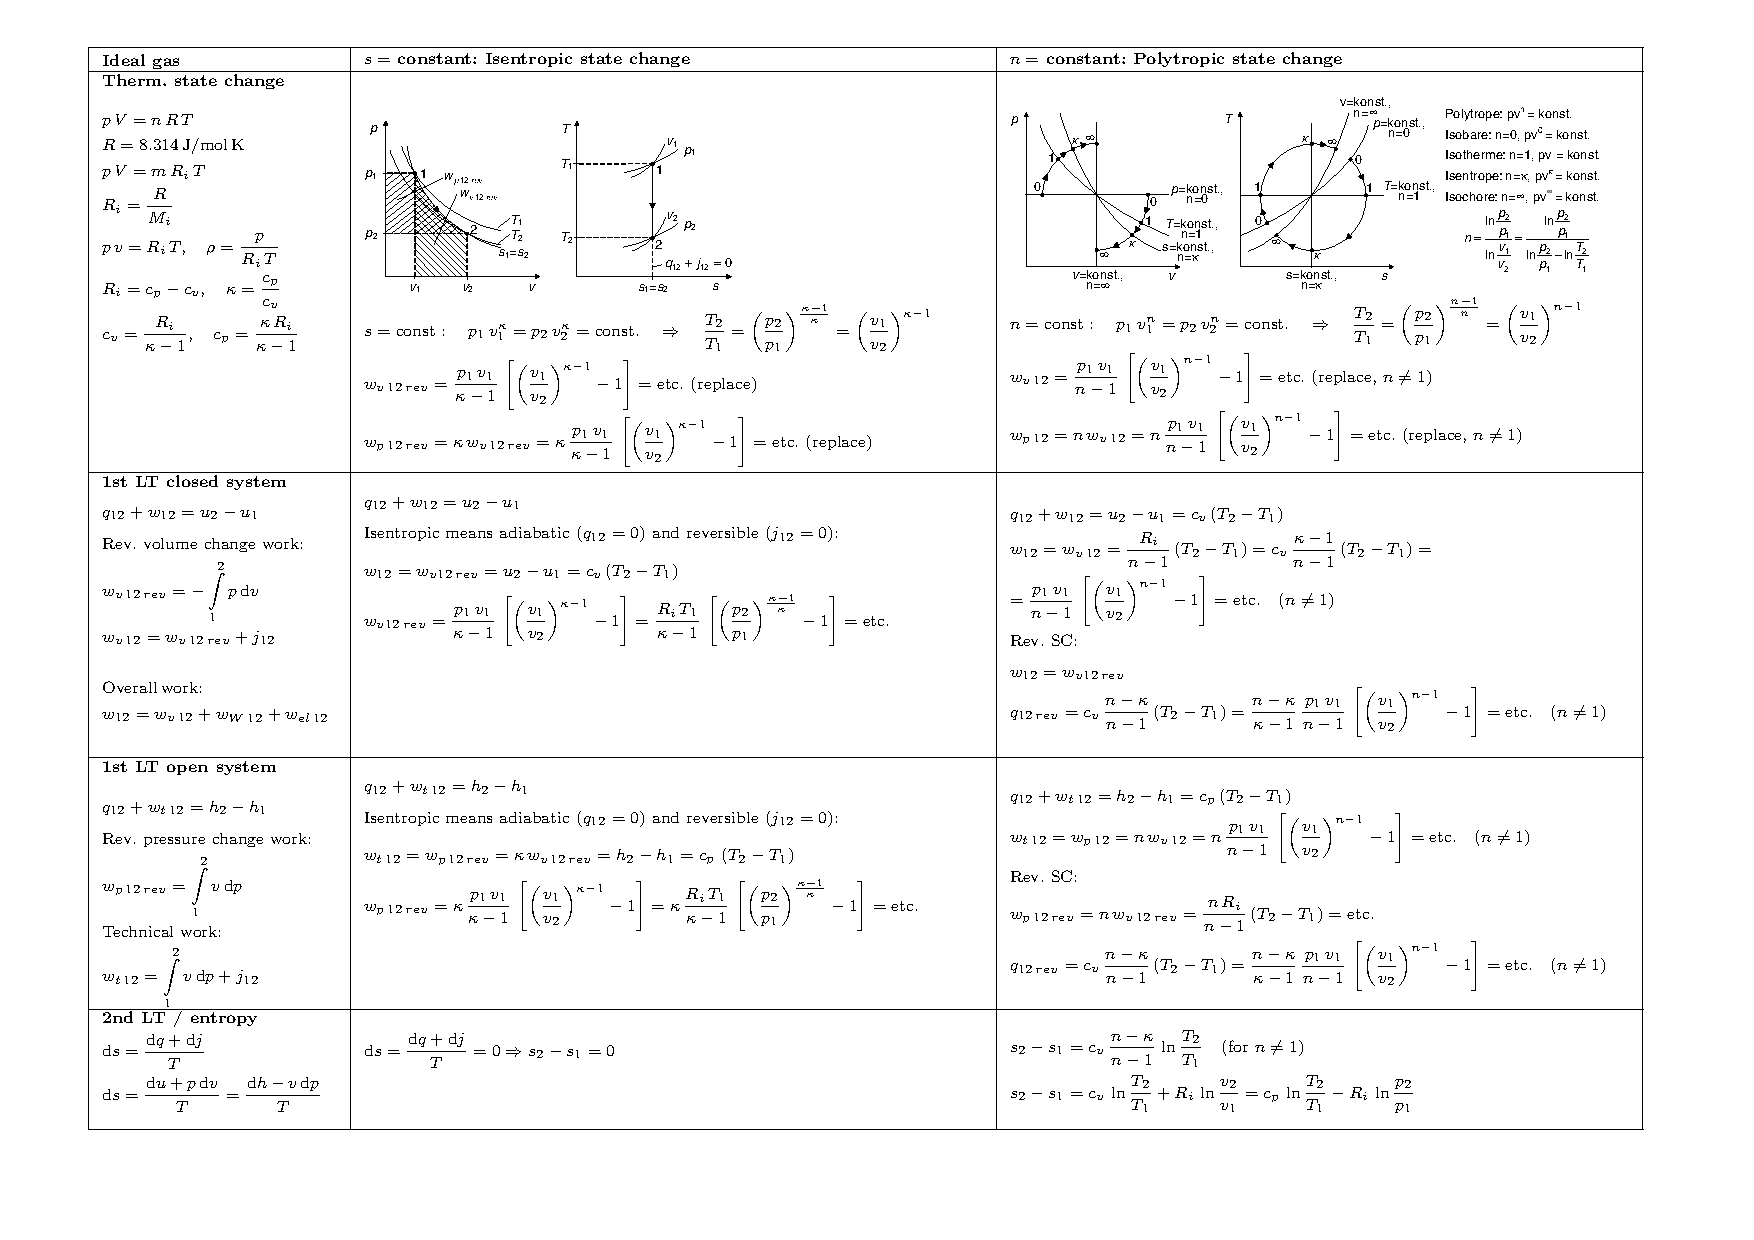
\includepdf[pages=1,pagecommand={\thispagestyle{fancy}}]{media/FormulaSheet-2.pdf}

\clearpage
\begin{multicols*}{3}
\raggedcolumns
\footnotesize
\section{Heat transfer: Mashing}
Malt and water are mixed in a mash tank. Hot water flows through a half-pipe
coil and heats the mash to $80^\circ C$.

\textbf{\underline{Data}}:
\begin{center}
\setlength{\tabcolsep}{3pt}
\renewcommand{\arraystretch}{1.2}
\begin{tabular}{@{}lll@{}}
  $m_m=100\,kg$ & $m_W=400\,kg$ & $\dot m_{HW}=0.4\,kg/s$\\
  $\vartheta_m=58^\circ C$ & $\vartheta_W=65^\circ C$ &
  $\vartheta_{HW,\alpha}=100^\circ C$\\
  $c_{pm}=3.57$ & $c_{pW}=4.2$ & $[kJ/(kgK)]$\\
  $Pr=4$ & $\nu_{HW}=2\cdot10^{-7}\,m^2/s$ &
  $\lambda_{HW}=0.6\,W/(mK)$\\
  $\rho_{HW}=1000\,kg/m^3$ & $\lambda_s=30\,W/(mK)$ & $D=1\,m$\\
  $r_i=35\,mm$ & $\delta=5\,mm$ & $\alpha_i=2000\,W/(m^2K)$
\end{tabular}
\end{center}
\renewcommand{\arraystretch}{1}

\subsection*{a\symbol{41}}
Calculate the initial mixed temperature $\vartheta_\text{mix}$, then the heat
needed to warm the mixture to $80^\circ C$.
\begin{gather*}
  \vartheta_\text{mix} =
  \frac{m_m c_{pm}\vartheta_m + m_W c_{pW}\vartheta_W}
  {m_m c_{pm}+m_W c_{pW}}
  =63.77^\circ C\\
  Q =
  \left(m_m c_{pm}+m_W c_{pW}\right)
  \left(80-\vartheta_\text{mix}\right)
  =33.05\,MJ
\end{gather*}

\subsection*{b\symbol{41}}
Sketch $\dot Q$ over heating time. Since the mash gets warmer, the temperature
difference to the hot water gets smaller, therefore $\dot Q$ decreases.

At $t_2$, $\vartheta_{HW,\alpha}$ is still $100^\circ C$, but
$\vartheta_{HW,\omega}$ is higher than at $t_1$ because less heat is transferred.
The mash temperature is nearly constant over one pass.

\begin{center}
\setlength{\tabcolsep}{3pt}
\begin{tabular}{@{}cc@{}}
\begin{minipage}{.48\linewidth}
\centering
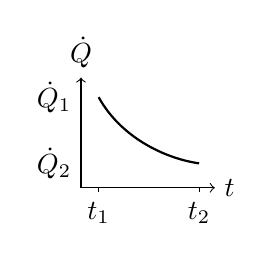
\begin{tikzpicture}[scale=.5]
  \draw[->] (0,0) -- (3.4,0) node[right] {$t$};
  \draw[->] (0,0) -- (0,2.8) node[above] {$\dot Q$};
  \draw[thick] (.45,2.3) .. controls (1,1.3) and (2.1,.75) .. (3,.62);
  \node[left] at (0,2.3) {$\dot Q_1$};
  \node[left] at (0,.62) {$\dot Q_2$};
  \draw (.45,0) -- (.45,-.12) node[below] {$t_1$};
  \draw (3,0) -- (3,-.12) node[below] {$t_2$};
\end{tikzpicture}
\end{minipage}
&
\begin{minipage}{.48\linewidth}
\centering
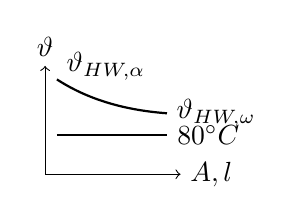
\begin{tikzpicture}[scale=.43]
  \draw[->] (0,0) -- (4,0) node[right] {$A,l$};
  \draw[->] (0,0) -- (0,3.2) node[above] {$\vartheta$};
  \draw[thick] (.35,1.15) -- (3.6,1.15) node[right] {$80^\circ C$};
  \draw[thick] (.35,2.8) .. controls (1.2,2.25) and (2.25,1.9) .. (3.6,1.8);
  \node[above right] at (.35,2.5) {$\vartheta_{HW,\alpha}$};
  \node[right] at (3.6,1.8) {$\vartheta_{HW,\omega}$};
\end{tikzpicture}
\end{minipage}
\end{tabular}
\end{center}

\subsection*{c\symbol{41}}
At $t_2$, $\dot Q=5\,kW$. Design the heat-transfer area using the half-pipe
Nusselt correlation and treat the half-pipe as a flat plate for $k$.
\begingroup
\scriptsize
\begin{align*}
  & A = \dfrac{r_i^2\pi}{2}=0.0019\,m^2\\[.8ex]
  & \dot V = \dfrac{\dot m}{\rho}=4\cdot10^{-4}\,m^3/s\\[.8ex]
  & v = \dfrac{\dot V}{A}=0.21\,m/s\\[.8ex]
  & Re = \dfrac{vL}{\nu}=\dfrac{v\pi r_i}{\nu}=115743\,[-]\\[.8ex]
  & Nu = 0.0214\left(Re^{0.8}-100\right)Pr^{0.4}
  \left[1+{\left(\dfrac{L_\text{char}}{D}\right)}^{2/3}\right]=510.37\\[.8ex]
  & \alpha = \dfrac{Nu\cdot\lambda_{HW}}{L_\text{char}}
   = \dfrac{Nu\cdot\lambda_{HW}}{\pi r_i}=2785\,W/(m^2K)
\end{align*}
\begin{align*}
  & k^{-1} = \dfrac{1}{\alpha_i}+\dfrac{\delta}{\lambda_s}+\dfrac{1}{\alpha}\\[.8ex]
  & k = \dfrac{1}{k^{-1}}=975\,W/(m^2K)\\[.8ex]
  & \dot Q = \dot m_{HW}c_{pW}
  \left(\vartheta_{HW,\alpha}-\vartheta_{HW,\omega}\right)
  \Longrightarrow \vartheta_{HW,\omega} = \vartheta_{HW,\alpha}
  - \dfrac{\dot Q}{\dot m_{HW}c_{pW}}\\[.6ex]
  & \vartheta_{HW,\omega}
  = 100^\circ C
  - \dfrac{\dot Q}{\dot m_{HW}c_{pW}}
  = 97^\circ C\\[.8ex]
  & \Delta T_m
  = \dfrac{\Delta T_a-\Delta T_b}{\ln\Delta T_a-\ln\Delta T_b}
   = \dfrac{\left(100-80\right)K-\left(97-80\right)K}
   {\ln\left(\frac{100-80}{97-80}\right)}
   = 18.5\,K\\[.8ex]
  & A = \dfrac{\dot Q}{k\Delta T_m}
   = 0.278\,m^2
\end{align*}
\endgroup

\section{2nd LT: Exergy of Thermal Energy Storages}
Two identical tanks store the same heat amount, either in serial
($T_{S,A}>T_P>T_{S,B}$) or in parallel ($T_{P,A}=T_{P,B}$), with homogeneous
tank temperatures.

\textbf{\underline{Data}}:
\begin{center}
\setlength{\tabcolsep}{3pt}
\renewcommand{\arraystretch}{1.2}
\begin{tabular}{@{}lll@{}}
  Serial mode & $T_{S,A}=90^\circ C$ & $T_{S,B}=50^\circ C$\\
  Parallel mode & $T_{P,A}=70^\circ C$ & $T_{P,B}=70^\circ C$\\
  Ambience & $T_{amb}=20^\circ C=293\,K$ & \\
  Water & $c_{p,W}=4200\,J/(kgK)$ & $=4.2\,kJ/(kgK)$
\end{tabular}
\end{center}
\renewcommand{\arraystretch}{1}

\subsection*{a\symbol{41}}
Calculate the specific energy content above $T_{amb}$ per $kg$ of water for each
tank in both cases.
\begingroup
\scriptsize
\begin{align*}
  & \boxed{u = c_{p,W}\left(T-T_{amb}\right)}\\[.8ex]
  & u_{S,A}=4.2\,kJ/(kgK)\cdot70\,K=294\,kJ/kg\\[.8ex]
  & u_{S,B}=4.2\,kJ/(kgK)\cdot30\,K=126\,kJ/kg\\[.8ex]
  & u_{P,A}=u_{P,B}=4.2\,kJ/(kgK)\cdot50\,K=210\,kJ/kg
\end{align*}
\endgroup

\subsection*{b\symbol{41}}
Calculate the specific entropy difference $s_{S,i}-s_{P,i}$ between serial and
parallel operation for both tanks. Water is incompressible, therefore
$c_v=c_p$.
\begingroup
\scriptsize
\begin{align*}
  & \boxed{s_{S,i}-s_{P,i}=c_{p,W}\ln\left(\dfrac{T_{S,i}}{T_{P,i}}\right)+\cancel{R_i\ln \left(\dfrac{v_2}{v_1}\right)}}\\[.8ex]
  & s_{S,A}-s_{P,A}=4.2\,kJ/(kgK)\ln\left(\dfrac{90+273}{70+273}\right)
  =0.24\,kJ/(kgK)\\[.8ex]
  & s_{S,B}-s_{P,B}=4.2\,kJ/(kgK)\ln\left(\dfrac{50+273}{70+273}\right)
  =-0.25\,kJ/(kgK)
\end{align*}
\endgroup

\subsection*{c\symbol{41}}
Calculate the specific exergy difference $e_{S,i}-e_{P,i}$ between serial and
parallel operation for both tanks.
\begingroup
\scriptsize
\begin{align*}
  & \boxed{e_{S,i}-e_{P,i} = h_{S,i}-h_{P,i}-T_{amb}\left(s_{S,i}-s_{P,i}\right)}\\[.8ex]
  & e_{S,A}-e_{P,A}
  = c_{p,W}\left(T_{S,A}-T_{P,A}\right)
  -T_{amb}\left(s_{S,A}-s_{P,A}\right)
  =13.68\,kJ/kg\\[.8ex]
  & e_{S,B}-e_{P,B}
  = c_{p,W}\left(T_{S,B}-T_{P,B}\right)
  -T_{amb}\left(s_{S,B}-s_{P,B}\right)
  =-10.75\,kJ/kg\\[.8ex]
  & e_S-e_P=\Delta e_A+\Delta e_B
  =\left(13.68-10.75\right)\,kJ/kg=2.93\,kJ/kg
\end{align*}
\endgroup

\section{2nd LT: Exergy Loss of Heat Transfer}
Heat flow through a wall from system A to B for three temperature pairs.

\textbf{\underline{Data}}:
\begin{center}
\setlength{\tabcolsep}{3pt}
\renewcommand{\arraystretch}{1.2}
\begin{tabular}{@{}lll@{}}
  $\dot Q=100\,kW$ & $T_E=T_{amb}=300\,K$ & \\
  i & $T_A=380\,K$ & $T_B=360\,K$\\
  ii & $T_A=380\,K$ & $T_B=340\,K$\\
  iii & $T_A=360\,K$ & $T_B=340\,K$
\end{tabular}
\end{center}
\renewcommand{\arraystretch}{1}

\subsection*{a\symbol{41}}
Formulate the exergy balance of the wall at steady state and derive the exergy
loss.
\begingroup
\scriptsize
\begin{align*}
  & \dot E_L=\sum_i\dot E_{x,i}-\sum_j\left|\dot E_{w,j}\right|
  =\dot Q\dfrac{T_A-T_E}{T_A}
  -\dot Q\dfrac{T_B-T_E}{T_B}\\[.8ex]
  & \boxed{\dot E_L
  =T_E\dot S_{irr}
  =T_E\dfrac{T_A-T_B}{T_AT_B}\dot Q}
\end{align*}
\endgroup

\subsection*{b\symbol{41}}
Calculate the exergy loss flow $\dot E_L$ for all three cases.
\begingroup
\scriptsize
\begin{align*}
  & \dot E_{L,i}
  =300\,K\cdot\dfrac{(380-360)\,K}{380\,K\cdot360\,K}\cdot100\,kW
  =4.4\,kW\\[.8ex]
  & \dot E_{L,ii}
  =300\,K\cdot\dfrac{(380-340)\,K}{380\,K\cdot340\,K}\cdot100\,kW
  =9.3\,kW\\[.8ex]
  & \dot E_{L,iii}
  =300\,K\cdot\dfrac{(360-340)\,K}{360\,K\cdot340\,K}\cdot100\,kW
  =4.9\,kW
\end{align*}
\endgroup

\subsection*{c\symbol{41}}
Calculate the entropy production $\dot S_{irr}$ for each case.
\begingroup
\scriptsize
\begin{align*}
  & \dot E_L=T_E\dot S_{irr}
  \Longrightarrow \dot S_{irr}=\dfrac{\dot E_L}{T_E}\\[.8ex]
  & \dot S_{irr,i}=\dfrac{4400\,W}{300\,K}=14.7\,W/K\\[.8ex]
  & \dot S_{irr,ii}=\dfrac{9300\,W}{300\,K}=31\,W/K\\[.8ex]
  & \dot S_{irr,iii}=\dfrac{4900\,W}{300\,K}=16.3\,W/K
\end{align*}
\endgroup

\newcolumn
\section{Stationary flow processes: Compressed-Air Energy Storage}
CAES stores electrical energy by compressing air into a cavern; a separate
turbine generates power during discharge.

\textbf{\underline{Data}}:
\begin{center}
\setlength{\tabcolsep}{2pt}
\renewcommand{\arraystretch}{1.2}
\begin{tabular}{@{}ll@{}}
  $\dot m_{air}=7200\,kg/h=2\,kg/s$ & $T_{2s}=579\,K$\\
  $p_1=p_5=1\,bar$ & $p_2=p_3=p_4=10\,bar$\\
  $T_1=T_3=300\,K$ & $T_2=T_4$\\
  $n_{comp}=1.5$ & $n_{exp}=1.3,\ \kappa=1.4$\\
  $c_{p,air}=1.004\,kJ/(kgK)$ & $R_{air}=287\,J/(kgK)$\\
  $c_{p,stone}=1.5\,kJ/(kgK)$ &
\end{tabular}
\end{center}
\renewcommand{\arraystretch}{1}

\textbf{Assumptions}: adiabatic compression/expansion with dissipation,
polytropic process, ideal thermal storage with $T_2=T_4$.

\subsection*{a, b\symbol{41}}
Draw and comment the state points in the $T,s$-diagram.
\begingroup
\scriptsize
\begin{align*}
  & T_2=T_1\left(\dfrac{p_2}{p_1}\right)^{(n_{comp}-1)/n_{comp}}
  =300\,K\cdot10^{0.5/1.5}=646\,K\\[.8ex]
  & T_2=T_4\\[.8ex]
  & T_5=T_4\left(\dfrac{p_5}{p_4}\right)^{(n_{exp}-1)/n_{exp}}
  =646\,K\cdot0.1^{0.3/1.3}=380\,K\\[.8ex]
  & 1\rightarrow2:\ \text{polytropic compression},\quad
  2\rightarrow3:\ \text{heat to storage}\\
  & 3\rightarrow4:\ \text{heat from storage},\quad
  4\rightarrow5:\ \text{polytropic expansion}
\end{align*}
\begin{center}
  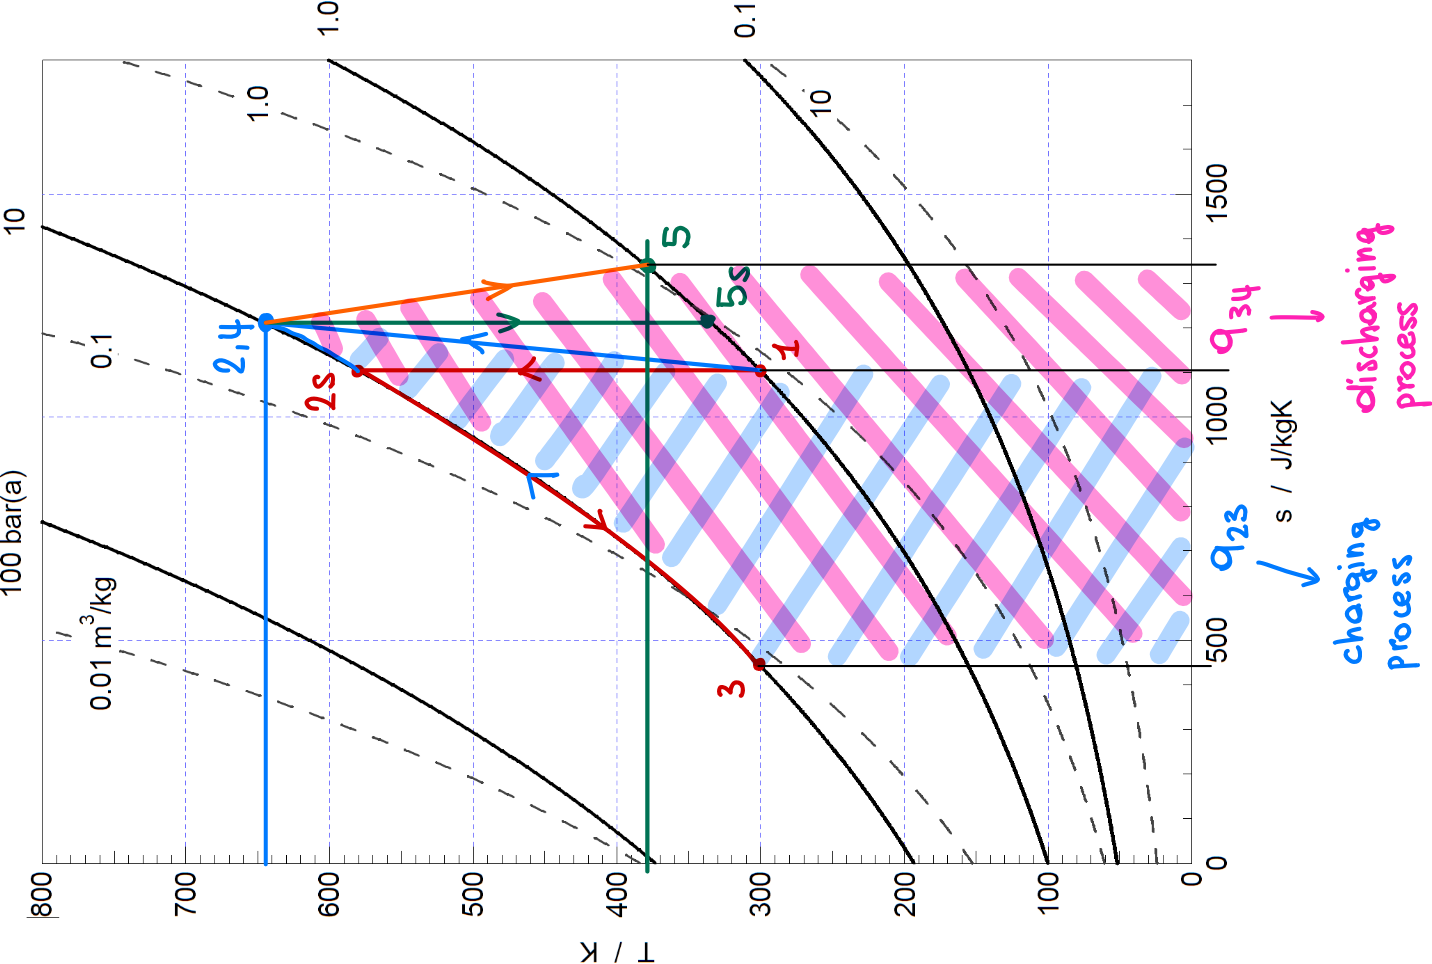
\includegraphics[\lw=.75]{media/ex-stationary.png}
\end{center}
\endgroup

\subsection*{c\symbol{41}}
Calculate the technical work and power of the compressor.
\begingroup
\scriptsize
\begin{align*}
  & w_{t,12}=h_2-h_1=c_{p,air}\left(T_2-T_1\right)=347.4\,kJ/kg\\[.8ex]
  & P_{12}=w_{t,12}\dot m_{air}=347.4\,kJ/kg\cdot2\,kg/s=694.8\,kW
\end{align*}
\endgroup

\subsection*{d\symbol{41}}
Calculate the technical work and power of the turbine.
\begingroup
\scriptsize
\begin{align*}
  & w_{t,45}=h_5-h_4=c_{p,air}\left(T_5-T_4\right)=-267.1\,kJ/kg\\[.8ex]
  & P_{45}=\left|w_{t,45}\right|\dot m_{air}
  =267.1\,kJ/kg\cdot2\,kg/s=534.1\,kW
\end{align*}
\endgroup

\subsection*{e\symbol{41}}
Calculate the isentropic efficiency of the compression.
\begingroup
\scriptsize
\begin{align*}
  & \eta_{s,C}=\dfrac{T_{2s}-T_1}{T_2-T_1}
  =\dfrac{579\,K-300\,K}{646\,K-300\,K}=0.806\,[-]
\end{align*}
\endgroup

\subsection*{f\symbol{41}}
For $4000\,kWh$ of mechanical energy, calculate the required thermal storage
energy.
\begingroup
\scriptsize
\begin{align*}
  & P_{34}=\dot m_{air}c_{p,air}\left(T_4-T_3\right)=694.8\,kW\\[.8ex]
  & t_{45}=\dfrac{E_{el}}{P_{45}}=\dfrac{4000\,kWh}{534.1\,kW}=7.489\,h\\[.8ex]
  & Q_{th}=P_{34}t_{45}=694.8\,kW\cdot7.489\,h
  =5203\,kWh=1.87\cdot10^7\,kJ
\end{align*}
\endgroup

\subsection*{g\symbol{41}}
Calculate the required storage mass for stones/gravel.
\begingroup
\scriptsize
\begin{align*}
  & Q_{th}=mc_{p,stone}\Delta T
  \Longrightarrow
  m=\dfrac{Q_{th}}{c_{p,stone}\Delta T}=36.03\,t
\end{align*}
\endgroup

\subsection*{h\symbol{41}}
Calculate the necessary cave volume at $p=10\,bar$.
\begingroup
\scriptsize
\begin{align*}
  & pV=mR_{air}T
  \Longrightarrow
  V=\dfrac{\dot m_{air}t_{45}R_{air}T_3}{p}
  =4642.6\,m^3
\end{align*}
\endgroup

\subsection*{i\symbol{41}}
Calculate the roundtrip efficiency.
\begingroup
\scriptsize
\begin{align*}
  & \eta_{RT}=\dfrac{\left|w_{out}\right|}{w_{in}}
  =\dfrac{\left|w_{t,45}\right|}{w_{t,12}}
  =\dfrac{267.1\,kJ/kg}{347.4\,kJ/kg}=0.769=76.9\%
\end{align*}
\endgroup

\subsection*{j\symbol{41}}
Choose whether to improve the compressor or turbine.

Improve the turbine: it increases the useful output directly, and for the same
stored heat and air mass this gives the strongest improvement of delivered
electricity and roundtrip efficiency.

\newcolumn
\section{Gas/Steam Turbines: Micro Steam Turbine}
High-pressure superheated steam is expanded from $15\,bar$ to $2\,bar$ in a
micro steam turbine instead of a throttling valve. Steam tables are used for the
property values; the $T,s$-graph is attached separately.

\textbf{\underline{Data}}:
\begin{center}
\setlength{\tabcolsep}{2pt}
\renewcommand{\arraystretch}{1.2}
\begin{tabular}{@{}ll@{}}
  $p_3=15\,bar(a)$ & $p_4=2\,bar(a)$\\
  $\dot m_s=6\,t/h=1.67\,kg/s$ & $\vartheta_3=250^\circ C$\\
  $\eta_s=0.8$ & $\eta_m=0.9,\ \eta_g=0.96$\\
  $P_{el,p}=20\,kW$ & $\eta_p=0.8,\ c_p=4.2\,kJ/(kgK)$\\
  $T_1=120.23^\circ C$ & $h_3=2923.5\,kJ/kg$\\
  $s_3=6.7099\,kJ/(kgK)$ & $h'=504.7,\ h''=2706.3\,kJ/kg$\\
  $s'=1.5301$ & $s''=7.1268\quad [kJ/(kgK)]$
\end{tabular}
\end{center}
\renewcommand{\arraystretch}{1}

\subsection*{a\symbol{41}}
Determine the temperature $T_2$ after the feedwater pump.
\begingroup
\scriptsize
\begin{align*}
  & P_{el,p}=\dfrac{\dot m_sc_p\Delta T}{\eta_p}
  \Longrightarrow
  \Delta T=\dfrac{P_{el,p}\eta_p}{\dot m_sc_p}\\[.8ex]
  & T_2=T_1+\Delta T
  =120.23^\circ C+
  \dfrac{20\,kW\cdot0.8}{1.67\,kg/s\cdot4.2\,kJ/(kgK)}
  =122.5^\circ C
\end{align*}
\endgroup

\subsection*{b\symbol{41}}
Calculate the steam content after the isentropic expansion.
\begingroup
\scriptsize
\begin{align*}
  & x_{4s}=\dfrac{s_{4s}-s'}{s''-s'}
  =\dfrac{s_3-s'}{s''-s'}\\[.8ex]
  & x_{4s}
  =\dfrac{6.7099-1.5301}{7.1268-1.5301}
  =0.926=92.6\%
\end{align*}
\endgroup

\subsection*{c\symbol{41}}
Calculate the enthalpy $h_4$ after the polytropic expansion.
\begingroup
\scriptsize
\begin{align*}
  & h_{4s}=(1-x_{4s})h'+x_{4s}h''
  =2542.3\,kJ/kg\\[.8ex]
  & \eta_s=\dfrac{h_3-h_4}{h_3-h_{4s}}
  \Longrightarrow
  h_4=h_3-\eta_s\left(h_3-h_{4s}\right)\\[.8ex]
  & h_4=2923.5-0.8\left(2923.5-2542.3\right)
  =2618.54\,kJ/kg
\end{align*}
\endgroup

\subsection*{f\symbol{41}}
Calculate the specific cycle work of the micro steam turbine.
\begingroup
\scriptsize
\begin{align*}
  & w=w_t-w_p=\left(h_3-h_4\right)-\left(h_2-h_1\right)\\[.8ex]
  & w=\left(h_3-h_4\right)-c_p\left(T_2-T_1\right)\\[.8ex]
  & w=\left(2923.5-2618.54\right)-4.2\left(122.5-120.23\right)
  =295.43\,kJ/kg
\end{align*}
\endgroup

\subsection*{g\symbol{41}}
Calculate the electrical power output of the generator.
\begingroup
\scriptsize
\begin{align*}
  & P_g=\dot m_s\left(h_3-h_4\right)\eta_m\eta_g\\[.8ex]
  & P_g=1.67\,kg/s\cdot\left(2923.5-2618.54\right)\,kJ/kg
  \cdot0.9\cdot0.96=440\,kW
\end{align*}
\endgroup

\subsection*{h\symbol{41}}
Calculate the thermal efficiency of the micro steam turbine.
\begingroup
\scriptsize
\begin{align*}
  & \eta_{th}=\dfrac{w}{q_{23}}
  =\dfrac{w}{h_3-h_2}
  =\dfrac{295.43\,kJ/kg}{\left(2923.5-4.2\cdot120\right)\,kJ/kg}
  =0.122=12.2\%
\end{align*}
\endgroup

\subsection*{d,e\symbol{41}}
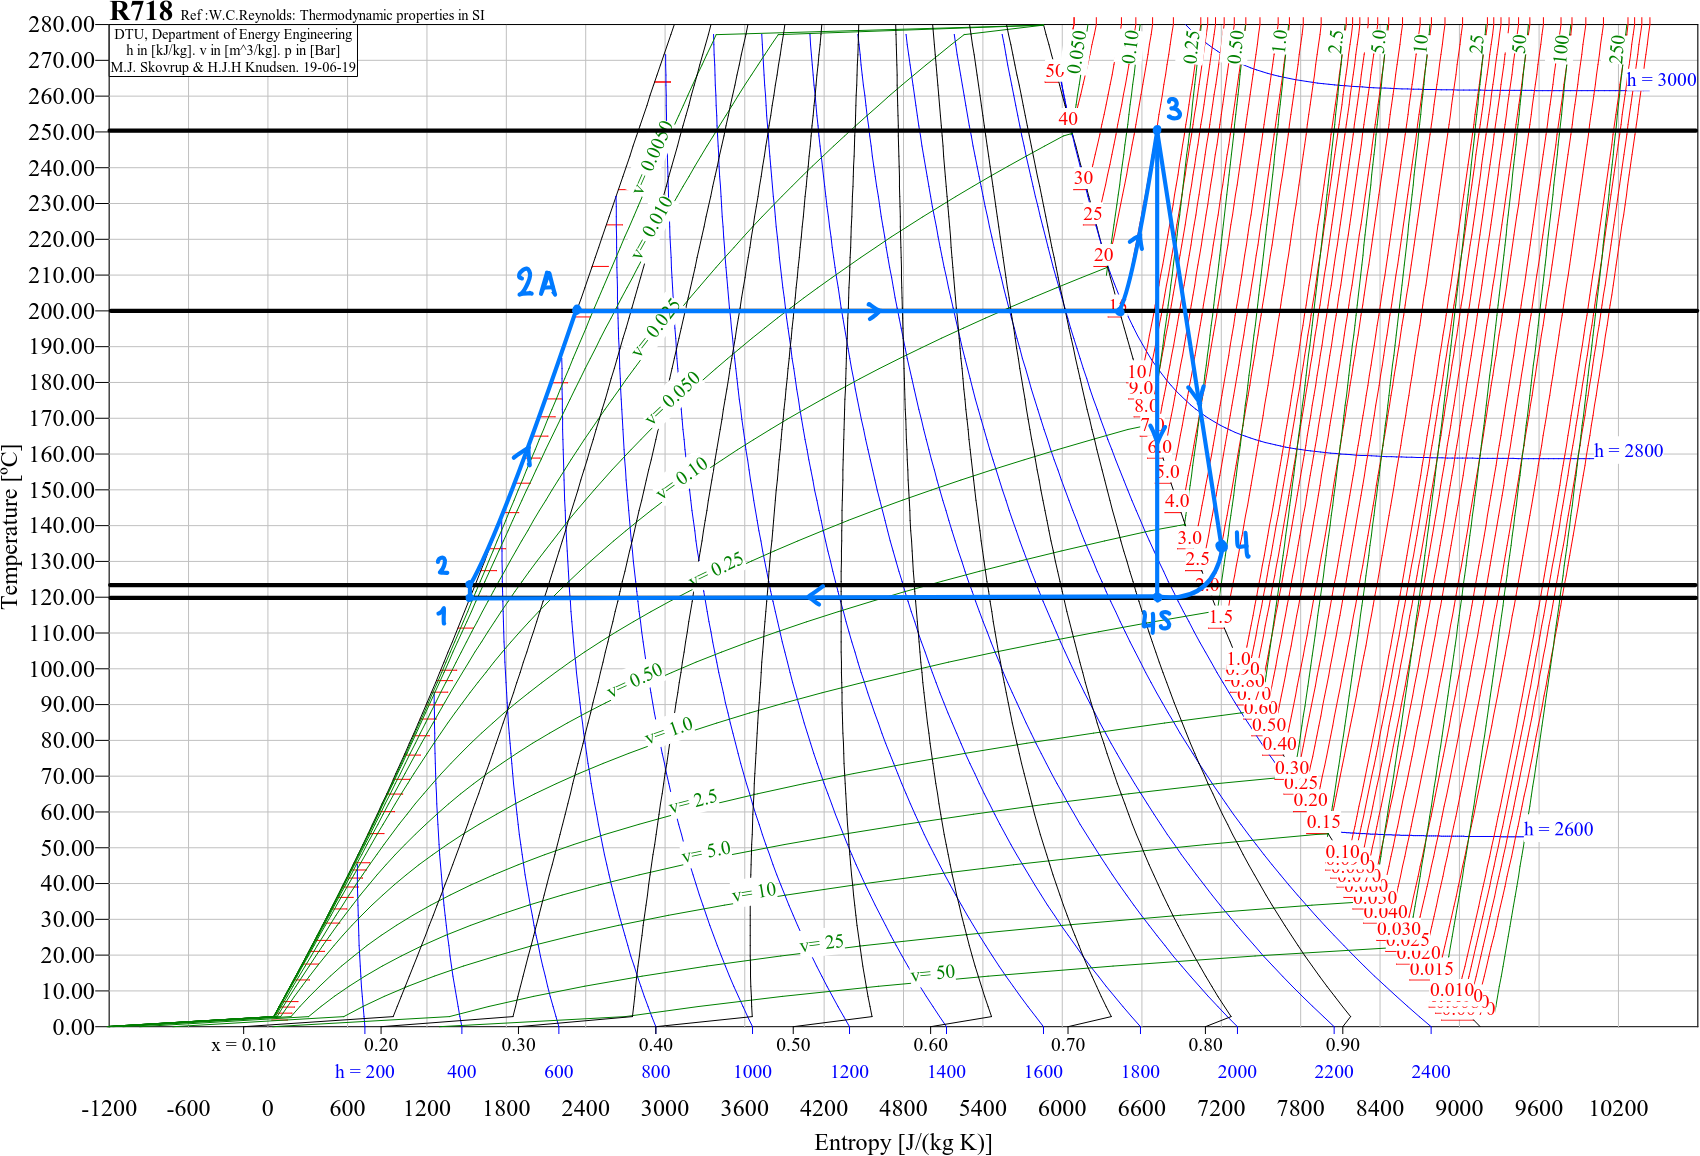
\includegraphics[\lw]{media/ex-steam.png}

\section{Heat Pumps: Decentralised Cooling System with Waterloop}
R290 cooling units reject condenser heat to a closed waterloop. The
waterloop releases the heat to ambient air through an air cooler.

\textbf{\underline{Data}}:
\begin{center}
\setlength{\tabcolsep}{2pt}
\renewcommand{\arraystretch}{1.2}
\begin{tabular}{@{}ll@{}}
  R290 propane & log $p,h$ diagram used separately\\
  $\eta_s=0.6$ & $\eta_{me}=0.92,\ P_{el}=1\,kW$\\
  $\Delta T_{SH}=7\,K$ & $\Delta T_{SC}=5\,K$\\
  $c_{p,W}=4.2\,kJ/(kgK)$ & $\rho_W=998\,kg/m^3$\\
  $\vartheta_{HW,\alpha}=35^\circ C$ & pump power neglected\\
  $\vartheta_{goods}=5^\circ C$ & $\vartheta_{amb}=23^\circ C$\\
  $\Delta T_E=10\,K$ & $\Delta T_C=5\,K,\ \Delta T_{AC}=3\,K$
\end{tabular}
\end{center}
\renewcommand{\arraystretch}{1}

\subsection*{a\symbol{41}}
Draw the cycle in the log $p,h$ diagram and fill in the state points.
\begingroup
\scriptsize
\begin{align*}
  & \vartheta_E=\vartheta_{goods}-\Delta T_E=5^\circ C-10\,K=-5^\circ C
  \Longrightarrow p_E\simeq4\,bar\\[.8ex]
  & \vartheta_C=\vartheta_{HW,\alpha}+\Delta T_C=35^\circ C+5\,K=40^\circ C
  \Longrightarrow p_C\simeq14\,bar\\[.8ex]
  & 1:\ p_E,\ \vartheta_1=\vartheta_E+\Delta T_{SH}=2^\circ C
  \Longrightarrow h_1\simeq580\,kJ/kg\\[.8ex]
  & 2s:\ p_C,\ s_{2s}=s_1
  \Longrightarrow \vartheta_{2s}\simeq52^\circ C,\ h_{2s}\simeq640\,kJ/kg\\[.8ex]
  & 2:\ \eta_s=\dfrac{h_{2s}-h_1}{h_2-h_1}
  \Longrightarrow h_2=h_1+\dfrac{h_{2s}-h_1}{\eta_s}
  \simeq680\,kJ/kg\\[.8ex]
  & 3:\ p_C,\ \vartheta_3=\vartheta_C-\Delta T_{SC}=35^\circ C
  \Longrightarrow h_3\simeq290\,kJ/kg\\[.8ex]
  & 4:\ h_4=h_3,\ p_E,\ \vartheta_4=\vartheta_E=-5^\circ C
\end{align*}
\endgroup
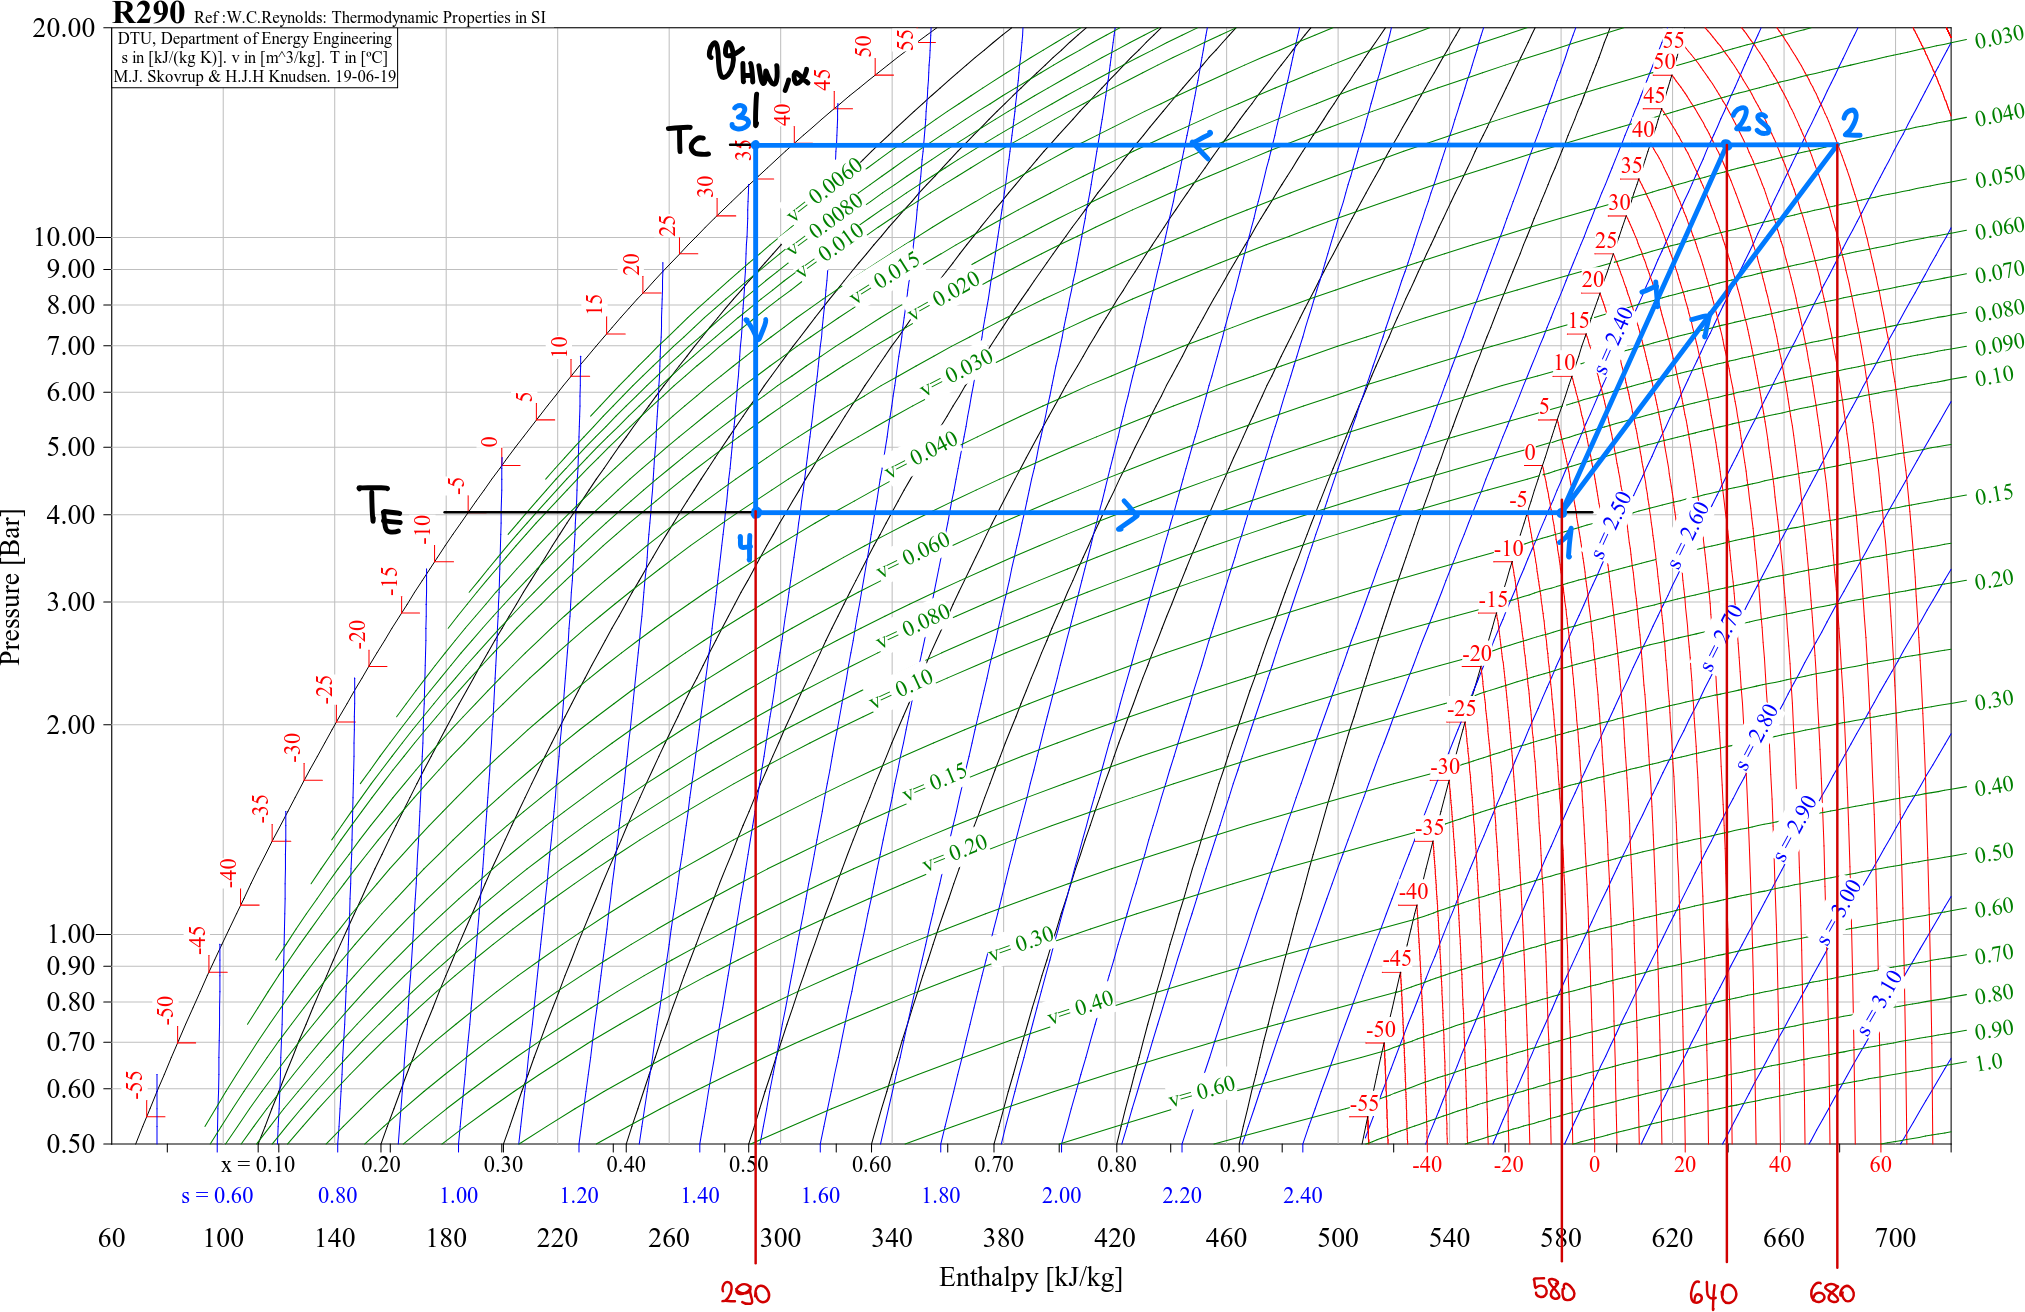
\includegraphics[\lw]{media/ex-hp.png}

\subsection*{b\symbol{41}}
Fill the table (by using the log p,h - diagram and calculations).
\begin{center}
\setlength{\tabcolsep}{3pt}
\renewcommand{\arraystretch}{1.15}
\begin{tabular}{|c|c|c|c|}
  \hline State point & $\vartheta\,[^\circ C]$ & $p\,[bar]$ & $h\,[kJ/kg]$\\
  \hline 1 & 2 & 4 & 580\\
  \hline 2 & 70 & 14 & 680\\
  \hline 2s & 52 & 14 & 640\\
  \hline 3 & 35 & 14 & 290\\
  \hline 4 & -5 & 4 & 290\\
  \hline 
\end{tabular}
\end{center}
\renewcommand{\arraystretch}{1}

\subsection*{c\symbol{41}}
Calculate the cooling capacity $\dot Q_E$ of one cooling unit.
\begingroup
\scriptsize
\begin{align*}
  & P_{el}\eta_{me}=\dot m\left(h_2-h_1\right)
  \Longrightarrow
  \dot m=\dfrac{P_{el}\eta_{me}}{h_2-h_1}
  =\dfrac{1\,kW\cdot0.92}{(680-580)\,kJ/kg}
  =0.0092\,kg/s\\[.8ex]
  & \dot Q_E=\dot m\left(h_1-h_4\right)
  =0.0092\,kg/s\cdot(580-290)\,kJ/kg
  =2.668\,kW
\end{align*}
\endgroup

\subsection*{d\symbol{41}}
Calculate the cooling-water volume flow for $\vartheta_{amb}=23^\circ C$.
\begingroup
\scriptsize
\begin{align*}
  & \dot Q_{23}=\dot m\left(h_2-h_3\right)
  =0.0092\,kg/s\cdot(680-290)\,kJ/kg=3.588\,kW\\[.8ex]
  & \dot V_{CW}
  =\dfrac{2\dot Q_{23}}{\rho_Wc_{p,W}\left(\vartheta_{HW,\alpha}-\vartheta_{amb}\right)}
  =\dfrac{2\cdot3.588\,kW}{998\,kg/m^3\cdot4.2\,kJ/(kgK)\cdot(35-23)\,K}\\
  & \dot V_{CW}=14.3\cdot10^{-5}\,m^3/s
\end{align*}
\endgroup

\subsection*{e\symbol{41}}
Evaluate the efficiency of one cooling unit.
\begingroup
\scriptsize
\begin{align*}
  & \varepsilon_C=\dfrac{T_E}{T_C-T_E}
  =\dfrac{-5+273}{(40+273)-(-5+273)}=5.96\\[.8ex]
  & \varepsilon_{CU}=\dfrac{h_1-h_4}{h_2-h_1}=2.9\\[.8ex]
  & COP_{CU}=\eta_{me}\varepsilon_{CU}=0.92\cdot2.9=2.668\\[.8ex]
  & \zeta_{CU}=\dfrac{COP_{CU}}{\varepsilon_C}=0.448
\end{align*}
\endgroup

\subsection*{f\symbol{41}}
Heating mode: parameters and expected effect.

The condenser temperature rises to supply building heating, therefore $p_C$ and
compressor work increase. The evaporator side is nearly unchanged, so the COP
decreases compared with summer operation.
\end{multicols*}

\end{document}
